% Options possibles
% init - pour le dossier d'initialisation
% francais ou english
% RandD - réservé aux PFE ayant le label R&D.
% Confidential - réservé aux PFE confidentiels
\documentclass[francais]{rapportPFE}  % pour une version française
%\documentclass[english]{rapportPFE}  % pour une version avec du texte en anglais

% L'option confidentiel a pour conséquence d'ajouter le filigrane "Confidentiel" sur la première et la dernière page
%  En fait, ce filigrane apparait sur toutes les pages numérotées 1 par Latex… 
% Pour le rajouter sur TOUTES les pages, décommenter la commande suivante
%\newwatermark[allpages,textalign=center,fontfamily=pbk,angle=55,scale=2.75,xpos=-1cm,ypos=1cm,color=lightgray]{Confidentiel}



\usepackage{listings}
\usepackage{fancyhdr}
\usepackage{caption} 
\usepackage{subfig}
\usepackage[skip=4pt plus1pt, indent=20pt]{parskip}
% %%%%%%%%%%%%%%%%%%%%%%%%%%%%%%%%%%%%%%%%%%%
% titres du rapport
% %%%%%%%%%%%%%%%%%%%%%%%%%%%%%%%%%%%%%%%%%%%
% Version francaise
\titre{Développement d'interface graphique technologie web - faisabilité et évaluation}
% version anglaise
\title{Development of web-based graphical user interface - feasibility and evaluation}


% %%%%%%%%%%%%%%%%%%%%%%%%%%%%%%%%%%%%%%%%%%%
% Auteur du rapport
% %%%%%%%%%%%%%%%%%%%%%%%%%%%%%%%%%%%%%%%%%%%
\firstname{Colin}
%\middlename{Autre-Prénom}
\lastname{Thomas}



% %%%%%%%%%%%%%%%%%%%%%%%%%%%%%%%%%%%%%%%%%%%
% Informations sur le PFE
% %%%%%%%%%%%%%%%%%%%%%%%%%%%%%%%%%%%%%%%%%%%
% Information administratives
\dateDebutPFE{5 février 2024}
\dateFinPFE{26 juillet 2024}
\nomStructureAcceuil{Arturia}
\villeStructureAccuel{Grenoble}
\logoStructureAccueil{width=5.0cm}{graphics/LogoStructureAccueil} % si vous ne souhaitez pas mettre de logo pour la structure d'accueil, commentez cette ligne.
% paramètres de la commande logoStructureAccueil
% #1 = paramètre d'affichage du logo
% #2 = nom du fichier logo
% Pour plus de précision, cela correspond à la commande latex \includegrahics[#1]{#2}

% Encadrants.
% Penser à accorder la fonction avec le genre
\begin{encadrants}
% Fonction {Fonction}{ Prénom \Nom{Nom}}{Titre}{Structure}
  \referent{Référent}{Yann \Nom{Gripay}}{Maître de Conférences}{INSA Lyon}%
  \tuteur{Tuteur}{Timothée \Nom{Béhéty}}{Référent Technique Logiciels Compagnon}{Arturia (Grenoble)}
\end{encadrants}

% Date de la soutenance
\date{26 juin 2024}

% Réglage des entêtes et pieds de page
\fancyhf{}
\renewcommand{\headrulewidth}{0.2pt}
\renewcommand{\footrulewidth}{0.2pt}
\fancyhead[L]{\footnotesize{Un exemple d'en-têtes 
     et pieds de page}}
\fancyfoot[R]{\thepage}
\fancyfoot[C]{\footnotesize{---}}
\fancyfoot[L]{\footnotesize{\textit{Les 
     rédacteurs de la FAQ}}}


% %%%%%%%%%%%%%%%%%%%%%%%%%%%%%%%%%%%%%%%%%%%
% Rapport lui même
% %%%%%%%%%%%%%%%%%%%%%%%%%%%%%%%%%%%%%%%%%%%
\begin{document}
\maketitle


% ==========================================
% les résumés et les mots clés du rapport
% ==========================================

\begin{ResumeMotsCles}

% Version anglaise
% abstract no more than 12 lines.
\begin{resumeEn}
During my final internship, I had the opportunity to participate in the design and development of web interfaces for Arturia's next generation Companion Softwares. These softwares include the Arturia Software Center, Arturia's software store, and the Midi Control Center, Arturia's hardware configuration software. With the aim of updating aging software and experimenting with new graphic development technologies, my team decided to prototype a modular application bringing them together, utilizing web interfaces for the front-end.\\
My role involved developing web interfaces for the Arturia Software Center, integrating a C++ back-end developed by another team member. I also redesigned the Midi Control Center and prototyped the use of the Web MIDI API to communicate with Arturia devices on the web, as well as experimenting with the Web USB API to update device firmware.\\
Throughout my internship, I followed and participated in the conception of the modular application during weekly architecture meetings. \\
Working on such an innovative project at Arturia allowed me to explore innovative domains and deepen my teamwork and communication skills, which I had developed during my previous internships. 
\end{resumeEn}
% keywords
\keywords{Web~; Vue Nuxt~; Cross-Plateform~; Web APIs~; Modular App.}



% Version francaise
% Résumé pas plus de 12 lignes
\begin{resumeFr}
Durant mon stage de fin d'études, j'ai pu participer à la conception et au développement d'interfaces Web pour la nouvelle génération des Logiciels Compagnon d'Arturia. Ces logiciels sont l'Arturia Software Center, le magasin de logiciels d'Arturia, et le Midi Control Center, le logiciel de configuration de matériel Arturia. Dans l'optique de mettre à jour des logiciels vieillissant, et d'expérimenter de nouvelles technologies de développement graphique, mon équipe a décidé de prototyper une application modulaire les rassemblant, et d'utiliser des interfaces Web pour la partie front-end. \\
Mon rôle a été de développer des interfaces Web pour l'Arturia Software Center, en y intégrant un back-end C++ développé par un autre membre de l'équipe. J'ai également réalisé un nouveau design pour le Midi Control Center, et ai pu prototyper l'utilisation de l'API Web MIDI pour communiquer avec les appareils Arturia.  \\
J'ai pu par ailleurs, au long de mon stage, suivre et participer à la conception de l'application modulaire lors de réunions d'architecture hebdomadaires.\\
Travailler sur un projet aussi innovant à Arturia m'a permis d'expérimenter des domaines novateurs, mais aussi d'approfondir mes compétences de travail en équipe et de communication que j'ai pu développer lors de mes précédents stages. 
\end{resumeFr}

% Mots clés
\motscles{Web~; Vue Nuxt~; Cross-Plateforme~; Web APIs~; Application Modulaire.}
\end{ResumeMotsCles}


% ==========================================
% Remerciements éventuels
% ==========================================
% \begin{remerciements}
%   Merci à tous. Commenter cet environnement s'il n'est pas nécessaire.
% \end{remerciements}





% %%%%%%%%%%%%%%%%%%%%%%%%%%%%%%%%%%%%%%%%%%
% rapport proprement dit 
% %%%%%%%%%%%%%%%%%%%%%%%%%%%%%%%%%%%%%%%%%%

% ==========================================
% Sommaire (généré automatiquement)
% ==========================================
\setcounter{tocdepth}{3}
\tableofcontents
\cleardoublepage

% ==========================================
% Introduction
% ==========================================
%Contexte, 
%définition du problème, 
%aperçu des contributions, 
%plan du rapport



     
     
     
\section{Introduction.}

\subsection{Mise en contexte.}
J'ai réalisé mon stage de fin d'études chez Arturia, une société Grenobloise, fabricant d'instruments de musique numériques et électroniques, du 5 février au 26 juillet 2024. C'était l'entreprise que je souhaitais intégrer pour ce stage de fin d'études, non seulement car j'utilise et apprécie les produits et logiciels Arturia, mais aussi car je souhaitais me rapprocher du milieu de ma passion pour la musique. 
J'ai intégré pendant ce stage l'équipe logiciel compagnon d'Arturia, qui m'a proposé un sujet de prototypage d'interfaces Web pour la nouvelle génération de deux de leurs logiciels, l'Arturia Software Center et le Midi Control Center. J'ai pu ainsi participer à la conception d'un logiciel modulaire rassemblant ces deux applications, développer des interfaces C++ préexistantes en Web, concevoir de nouvelles interfaces et prototyper l'utilisation d'APIs Web novatrices. Ce stage me permet de mettre en oeuvre les compétences de développement Web acquises pendant mon stage précédent, ainsi que de mettre en pratique les connaissances théoriques que j'ai pu apprendre pendant mes études, telles que la programmation, de technologies Web ou encore le génie logiciel.
\subsection{Définition du problème.}

Les logiciels Arturia sont séparables en deux catégories : les instruments et effets logiciels, qui créent et modifient de l'audio, et les logiciels Compagnon, qui accompagnent les produits vendus par Arturia.
L'Arturia Software Center (ASC) et le Midi Control Center (MCC) font partie de cette dernière, et sont respectivement le gestionnaire de logiciels et licenses, et le logiciel de configuration d'appareils physiques d'Arturia.

Arturia souhaite mettre à jour un Midi Control Center vieillissant et difficilement maintenable, tout en simplifiant son ecosystème logiciel ainsi qu'en modernisant les architectures techniques au sein de l'entreprise. Pour ce faire, l'entreprise a décidé fusionner ces deux logiciels en un seul, doté d'une architecture modulaire et d'interfaces basées sur les technologies Web. 

Le défi de mon équipe est donc de réussir à adapter un logiciel préexistant dans une nouvelle technologie, en séparant le front-end et le back-end qui était alors trop lié dans une architecture totalement C++, et en réussissant à faire une application suffisemment modulaire, maintenable et extensible pour qu'elle puisse intégrer à l'avenir de nouveaux éléments non encore définis.

Ainsi, mon défi personnel est de réussir à produire un prototype initial des interfaces Web pour ces deux logiciels, tout en expérimentant les possibilités d'utilisation du MIDI et de l'USB dans des technologies Web.



\subsection{Aperçu des contributions.}
% //TODO : mettre à jour
Lors de ce stage, j'ai pu travailler sur plusieurs éléments : 
\begin{itemize}
    \setlength\itemsep{0em}
    \item Démontrer l'utilisation de multiples Frameworks Web (React, Angular, Vue, Vue Nuxt) dans une application modulaire C++ Juce, ainsi que dans une application démo de Chromium Embedded Framework.
    \item Développer toutes les interfaces existantes C++ de l'Arturia Software Center en Vue Nuxt.
    \item Concevoir et développer les interfaces d'un Midi Control Center entièrement en Web, qui permet de configurer le clavier maître Arturia MiniLab 3.
    \item Concevoir et développer l'interface du logiciel modulaire accueillant le Midi Control Center et l'Arturia Software Center.
    \item Prototyper l'implémentation de l'API Web MIDI pour communiquer avec les appareil Arturia en front-end Web uniquement.
    \item Expérimenter l'utilisation de l'API Web USB pour mettre a jour un périphérique Arturia via le protocol standard USB DFU (Device Firmware Update).
    \item Participer activement à la conception et à l'architecture du projet tout entier, en étant force de proposition ainsi qu'en {{disant qu'est ce qui est possible ou pas}}.
\end{itemize}
La majeure partie de mon travail était concentrée sur le développement des interfaces Web du Midi Control Center, ainsi que de l'Arturia Software Center, en étroite collaboration avec Jean-Yves TISSOT, le developpeur C++ chargé de l'implementation du backend. 

\subsection{Problématique et plan.}

La problématique de ce rapport de stage concerne d'une part, l'intégration d'interfaces Web dans un logiciel modulaire, et d'autre part, l'objectif de déplacement de l'intelligence logicielle du Midi Control Center dans le Web, impliquant l'expérimentation et la démonstration d'utilisation de l'API de diverses technologies Web novatrices.

Dans ce rapport, je traiterai premièrement du contexte du stage, en présentant l'entreprise et l'équipe que j'ai intégré, ainsi que mon sujet de stage. Je poursuivrai par une analyse des deux logiciels sur lesquels j'ai travaillé, leurs fonctionnalités et leurs spécificités. Ensuite, je développerai les propositions techniques et implémentations que j'ai pu réaliser sur l'Arturia Software Center, le Midi Control Center, ainsi que les API Web que j'ai étudiés, en décrivant également la méthodologie de travail et l'environnement technique utilisé, ainsi que les expérimentations et validations réalisées au cours de ce stage.
% //TODO : plan


\section{Contexte.}

\subsection{Contexte du stage.}
\subsubsection{Intégration à l'équipe Compagnon}
Pour ce stage, j'ai été intégré à l'équipe Compagnon d'Arturia, une sous-équipe de l'équipe Système au sein du département R\&D. Sous la supervision de mon tuteur, Timothée Béhéty, qui dirige cette sous-équipe composée de 4 membres, j'ai étroitement collaboré avec Jean-Yves Tissot, responsable du développement du back-end C++ de l'Arturia Software Center (ASC) et est le développeur du projet GeMAPS. Puisque l'équipe Compagnon se concentre exclusivement sur le développement en C++, j'ai sollicité l'expertise de Fabian Boilay, membre de l'équipe de développement du site web d'Arturia, pour les revues de code. 


\begin{center}
	\centering
	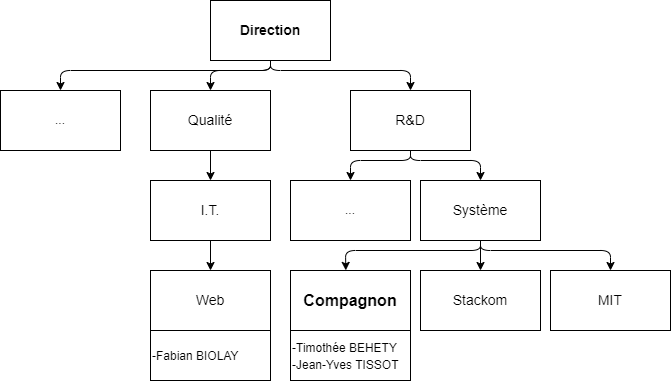
\includegraphics[width=0.8\textwidth]{graphics/organigramme.png}
	\begin{tiny}
	\end{tiny}
	\captionof{figure}{Organigramme simplifié d'Arturia : emplacement de l'équipe Logiciel Compagnon}
	\label{fig}
\end{center}

\subsubsection{Méthodologie.}
A COMPLETER

% méthodologie
% front-end ?


\subsection{Arturia.}

Arturia est un fabricant d'instruments de musique numériques et électroniques. La société est basée à Grenoble et développe des reproductions logicielles d'anciens synthétiseurs (analogiques et numériques), des claviers MIDI, des contrôleurs, des synthétiseurs analogiques et des interfaces audio. 

Il s'agit d'une entreprise employant 180 personnes, qui a été fondée en 1999. A sa création, ses deux fondateurs Frédéric Brun (actuel CEO d'Arturia) et Gilles Pommereuil ont commencé par créer des reproductions de synthétiseurs analogiques réputés au format virtuel, en commençant par développer ModularV, inspiré par les synthétiseurs Moog et en collaboration avec leur créateur. De nombreuses autres reproductions ont suivi, et sont devenues par la suite la V Collection, qui est la collection d'instruments virtuels d'Arturia, et la FX Collection, qui est son équivalent pour les effets audio.

Arturia a depuis élargi son catalogue à des instruments virtuels qui lui sont propres, mais c'est également lancé dans la conception de produits matériels, comme plusieurs synthétiseurs analogiques renommés, différents contrôleurs MIDI ainsi que des cartes sons. 

L'équipe Compagnon dans laquelle je réalise mon stage s'occupe des logiciels accompagnants les produits Arturia, comme le gestionnaire de licences, le logiciel de configuration de matériel, ou encore des logiciels spécifique à chaque produit, comme par exemple l'application mobile qui accompagne le clavier AstroLab. 

\subsection{Présentation du sujet de stage.}


\subsubsection{Mission.}

L'Arturia Software Center (ASC) et le Midi Control Center (MCC) sont deux logiciels vieillissants, qu'Arturia souhaite mettre à jour. Pour faire cela, l'entreprise souhaite mettre à l'épreuve de nouvelles technologies de développement graphique.

En effet, ces logiciels ont été développés respectivement en 2014 pour l'Arturia Software Center, et en 2013 pour le Midi Control Center. A ce moment, l'équipe Compagnon que j'intègre pour ce stage n'existait pas encore, et ces logiciels ont donc étés développés par l'équipe Software, qui se spécialise dans le développement d'instruments virtuels. Ils ont opté pour l'utilisation de technologies de développement d'instruments virtuels, notamment le framework C++ JUCE, pour la création de ces outils. Cependant, une mise à jour de l'ASC et du MCC en utilisant des technologies différentes permettrait de se détacher des outils spécifiquement conçus pour les logiciels audio, potentiellement inadaptés à ces applications.

Ainsi, l'équipe Compagnon a décidé de prototyper une application modulaire fusionnant l'Arturia Software Center et le Midi Control Center. L'architecture modulaire s'appellerait General Modular Architecture with Pluggable Services (GeMAPS) et son application au Midi Control Center et à l'Arturia Software Center se nommerait Unified Control Center (UCC). Cette application serait capable de lancer des librairies C++ en tant que back-end, de servir en HTTP des pages Web statiques en tant que front-end, et d'afficher un host permettant de naviguer sur ces pages Web. 


\begin{center}
	\centering
	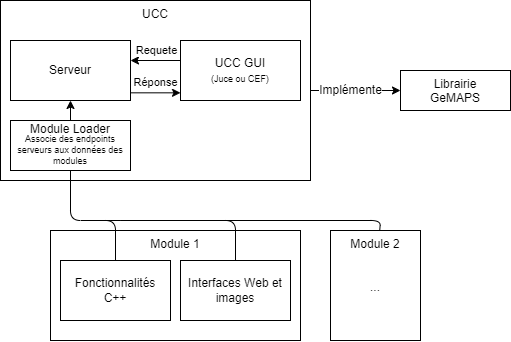
\includegraphics[width=0.5\textwidth]{graphics/modulaire.png}
	\begin{tiny}
	\end{tiny}
	\captionof{figure}{Architecture modulaire GeMAPS}
	\label{fig}
\end{center}

De cette manière, l'Arturia Software Center et le Midi Control Center constitueraient deux modules de cette application, chacun dotés d'un back-end sous forme de librairie C++, et d'un front end sous forme de page web statique, communiquant avec leur back-end par requêtes HTTP.\\

\subsubsection{Enjeux de ma mission.}

Utiliser des interfaces web pour ces logiciels se révèle ainsi positif sur plusieurs points : 
\begin{itemize}
	\item Les technologies web sont plus efficaces pour créer rapidement des interfaces. En effet, les bibliothèques et outils pré-développés et libres d'accès sont nombreux, en constante évolution, et faciles d'utilisation : on peut prendre pour exemple la fonctionnalité multilingue, qui est une fonctionnalité qui prend de l'importance pour Arturia, et qui demande beaucoup de ressources dans les applications C++, pour un développement plus facile, classique et très documenté en technologies Web. De même, les framework Web offrent souvent une courbe d'apprentissage plus faible que le C++ ou autre langage qui n'est pas haut-niveau.
	\item La fonctionnalité multilangue, qu'Arturia souhaite importer dans ses logiciels, est d'ores et déjà développée dans l'équipe de développement du site Web : en effet, l'équipe Web d'Arturia a, pendant les deux dernières années, réalisé un processus complexe de traduction de son site Web, avec envoi automatique du texte aux traducteurs, relectures... Utiliser les technologies Web de l'équipe de développement Web d'Arturia permettrait ainsi d'intégrer leur processus de traduction.
	\item Ceci permet, pour développer ces interfaces, de pouvoir rechercher des profils de développeurs front-end Web, puis de les former sur le framework JUCE, pour ensuite travailler sur des interfaces. En séparant le développement front-end du reste de l'application, ceci permet de rechercher des développeurs spécialisés dans leur domaines, et ainsi une meilleure évolutivité de l'équipe.
	\item Ensuite, cela permet de séparer le front-end du back-end. En effet, avoir une interface HTTP entre un back-end et un front-end permet de bien séparer ces deux parties. Ceci amène de la modularité et de la scalabilité, car chaque partie peut être modifiée sans affecter l'autre. On peut imaginer également une plus grande flexibilité technologique, car l'application Web pourrait être développée dans n'importe quel framework, sans impliquer de changement pour les librairies C++.
\end{itemize}

L'Arturia Software Center étant l'outil qui permet de gérer l'installation des logiciels, un back-end est forcément nécessaire pour soutenir le front-end. En effet, par design et pour des raisons de sécurités, les technologies Web n'ont pas accès au système de fichiers de l'utilisateur.

En revanche, la question se posera pour le Midi Control Center, dont la principale fonctionnalité est de communiquer par protocole Midi avec le contrôleur. Nous étudierons pendant ce stage la faisabilité d'un Midi Control Center entièrement réalisé en technologies Web.

\section{Etude bibliographique et analyse de l'existant.}


\subsection{Définitions nécessaires.}

Nous allons ici définir quelques termes propres au matériel de production musicale.
\paragraph{MIDI} \cite{midi}
: Le Musical Instrument Digital Interface ou MIDI est un protocole de communication défini dans les années 1980 dédié à la représentation de l'information musicale, et utilisé pour la communication entre instruments électroniques, contrôleurs, séquenceurs, et logiciels de musique. Il s'agit du protocole standard du matériel électronique de musique. Il permet par exemple à un Contrôleur MIDI d'envoyer le signal qu'une certaine note a été pressée avec une certaine vélocité, permettant à un logiciel sur ordinateur de produire un son en conséquence. Dans le sens inverse, ce protocole permet à l'utilisateur de paramétrer son contrôleur MIDI en envoyant des signaux SysEx, comportant les informations nécessaire sur le paramètre à modifier et la valeur à lui attribuer.
\paragraph{Message SysEx} \cite{sysex}
: Un message SysEx est un type de message MIDI permettant de régler les paramètres d'un périphérique MIDI, ce qui n'est pas adapté à la syntaxe normale du protocole MIDI. 
\paragraph{Contrôleur MIDI}  \cite{controller}
:  Un contrôleur MIDI est un appareil utilisé pour envoyer des signaux MIDI à l'ordinateur où à un autre appareil (par exemple, un synthétiseur analogique). Il peut se présenter sous la forme d'un clavier de piano, de faders, de potentiomètres, d'encodeurs, ou autres.
\paragraph{GeMAPS} : \textit{General Modular Application with Pluggable Software}. Il s'agit de l'architecture modulaire que l'on conçoit pendant ce stage, et qu'utilise le UCC.
\paragraph{UCC} : \textit{Unified Control Center}. C'est l'implémentation de GeMAPS pour l'Arturia Software Center.
% \paragraph{Synthétiseur analogique} \footnote{\url{https://fr.wikipedia.org/wiki/Synthétiseur_analogique}} 
% : Un synthétiseur analogique est un synthétiseur qui utilise des circuits analogiques et des signaux électriques analogiques pour générer des sons par des techniques électroniques. Contrairement à un synthétiseur numérique, qui stocke et communique l'information en binaire, l'information sonore est transmise dans l'analogique en tant que variation de tension.
% \paragraph{Synthétiseur virtuel :} Un synthétiseur analogique virtuel est un synthétiseur simulant le son de synthétiseurs analogiques par le biais de processeurs numérique. Il peut être utilisé sous la forme de Stand-Alone, c'est à dire sans logiciel qui l'entoure, en le contrôlant par exemple par un contrôleur MIDI, mais également et plus populairement sous la forme Plug-In, c'est à dire en tant que module à intégrer à un logiciel de Musique Assistée par Ordinateur.
\subsection{L'Arturia Software Center existant.}

L'Arturia Software Center \cite{asc}
 (ASC) est le logiciel de gestion de licences et de
téléchargement de logiciels d'Arturia : il est nécessaire pour tout utilisateur
souhaitant utiliser un logiciel Arturia. 

L'utilisateur, une fois connecté, peut naviguer parmi les logiciels disponibles sur l'Arturia Software Center sur la page "Explore Products", activer la licence du logiciel sur la page "My Products", le télécharger, le mettre à jour sur la page "My Updates", gérer l'emplacement de ses fichiers dans les paramètres, ainsi que de rentrer le code d'un produit Arturia physique afin de bénéficier des logiciels qui l'accompagnent.  Par ailleurs, s'il ne possède pas de connexion internet, il peut procéder à une activation hors-ligne.

L'Arturia Software Center est composé de deux parties : 

Tout d'abord, une partie principale, qui est ce logiciel qui permet de gérer ses licences et ses téléchargements de logiciels Arturia, et fournit une interface graphique.

Ensuite, un logiciel nommé ASC Agent, qui fonctionne en arrière plan, et vérifie les licences utilisateur à chaque démarrage de produit Arturia, afin d'éviter toute fraude et téléchargement illégal.

\begin{center}
	\centering
	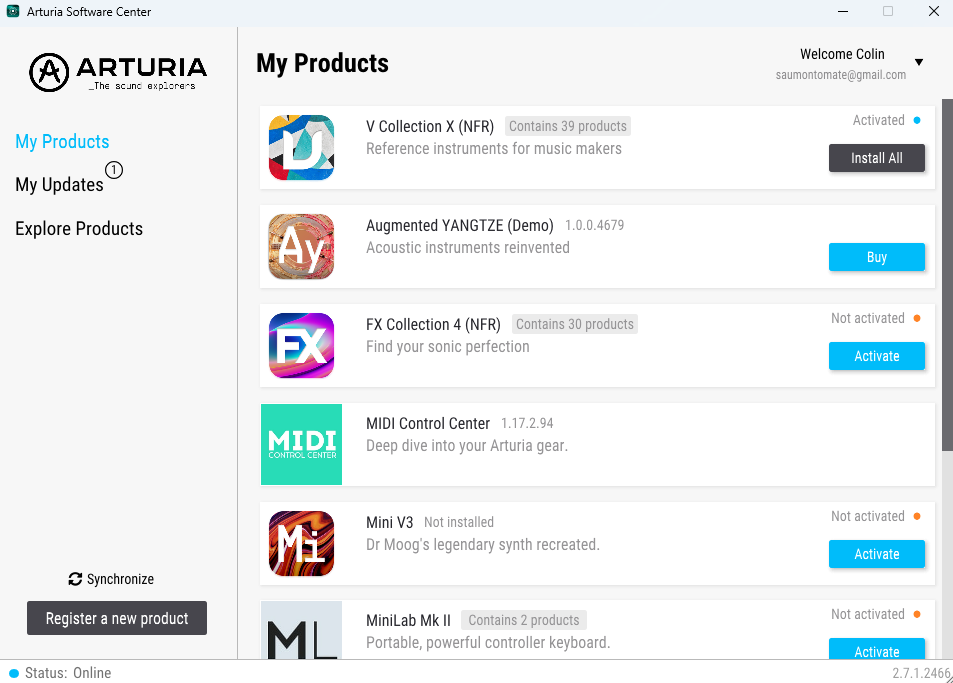
\includegraphics[width=0.6\textwidth]{graphics/asc_existant.png}
	\begin{tiny}
	\end{tiny}
	\captionof{figure}{Arturia Software Center (ASC) existant}
	\label{fig}
\end{center}

\subsection{Le Midi Control Center existant.}

Le Midi Control Center \cite{mcc}
 (MCC) est le logiciel de configuration de matériel Arturia : il
permet de gérer les configurations et les paramètres des synthétiseurs et contrôleurs MIDI, ainsi que de faire les mises à jour firmware pour les synthétiseurs analogiques, cartes sons et claviers LMIDI physiques d'Arturia. Il communique en norme MIDI avec les produits Arturia pour leur configuration.

Nous pouvons, sur ce logiciel, sélectionner un appareil Arturia parmis la liste proposée. Ceci affiche les fenêtres de paramètrage disponible pour le controleur sélectionné. Nous allons ici décrire les pages disponibles pour la série des controleurs MIDI de la gamme Lab, car c'est ceux sur lequels je me suis concentré pendant ce stage.

La page "Device Settings" est présente pour tous les controleurs. ELle permet de modifier les paramètres globaux du contrôleur actuellement connecté (par exemple, son temps de mise en veille ou ses courbes de vélocité).

La page "Controller Map" permet de modifier les paramètres de chaque contrôle du contrôleur, (par exemple, modifier la note attribuée à une touche en particulier).

Nous disposons également d'un menu permettant d'importer ou d'exporter des fichiers contenant les paramètres du contrôleur. Le logiciel effectue également une détection automatique de mises à jour disponibles pour le firmware du contrôleur. 

\begin{center}
	\centering
	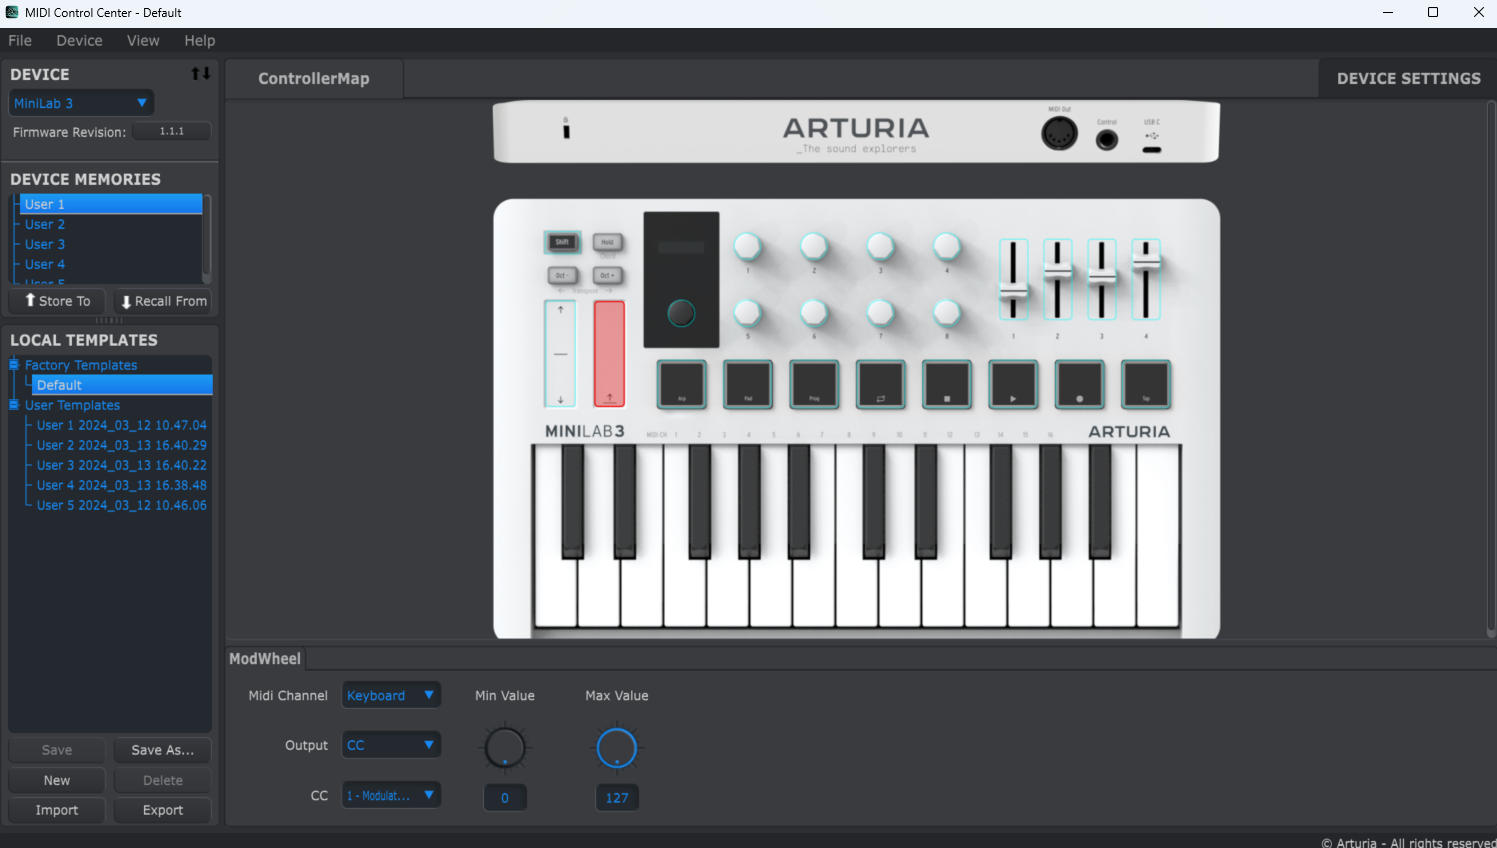
\includegraphics[width=0.6\textwidth]{graphics/mcc_existant.png}
	\begin{tiny}
	\end{tiny}
	\captionof{figure}{Midi Control Center (MCC) existant}
	\label{fig}
\end{center}

Tous les paramètres des appareils Arturia sont décrit dans des fichiers JSON, avec leur nom, si ils sont généraux ou spécifiques à un controle, ainsi que leur valeur par défaut. 

Les paramètres de controleurs MIDI de la gamme Lab sont regroupés en deux catégories :
\begin{itemize}
    \item Les paramètres d'appareils (Device Settings) sont des paramètres globaux, regroupés par catégories, qui comportent par exemple le temps de mise en veille, ou le mode de fonctionnement de la pédale. Ces paramètres sont récupérés au branchement de l'appareil. Ils sont mis à jour à chaque changement : dès que l'utilisateur modifie un paramètre, un message SysEx est envoyé à l'appareil.
    \item Les paramètres de préréglage (Preset Settings) sont des paramètres assignés à chaque contrôle de l'appareil. Par exemple, cela peut être la note assignée à un pad, ou le minimum et le maximum d'un slider. 
    
    Ceux-ci sont assignés à des "profils" : en fonction de l'appareil, certains sont prédéfinis et non modifiables, comme par exemple le profil DAW qui est compatible avec les logiciels de Musique Assistée par Ordinateur, tandis que d'autres sont personnalisables. Ainsi, on peut importer le profil que l'on désire depuis l'appareil, le modifier, puis le réinsérer dans le profil souhaité sur l'appareil. 

    Il est possible d'importer et d'exporter ces paramètres sur des fichiers locaux sur l'ordinateur. Ceci permet à l'utilisateur de sauvegarder un paramètrage de son clavier, ou encore le partager sur une autre unité. Les paramètres sont sauvegardés sous un format JSON, liant l'ID de chaque paramètre à sa valeur.
\end{itemize}

\subsection{Les API Web MIDI et Web USB.}

L'API Web MIDI \cite{webmidi1}
fournit une manière pour les applications web d'interagir avec les périphériques MIDI connectés à l'ordinateur. Elle permet d'envoyer et de recevoir des messages MIDI. Par exemple, dans notre cas préci, nous pouvons recevoir des messages de Note On / Note Off, mais aussi envoyer des messages SysEx permettant de modifier les paramètres du périphérique.

Cette API existe depuis plus de 10 ans, et est supportée par l'organisme de standardisation W3C. Elle est cependant encore en stade de développement, et bien qu'elle ai été supportée par l'organisme de standardisation W3C, celui-ci ne l'a pas standardisée \cite{webmidi2}. Cela signifie que son soutien par les navigateurs n'est pas obligatoire. Actuellement, cette API n'est disponible que sur les navigateurs Safari et Chromium. Cependant, cela ne pose aucun problème pour notre application, car nous avons la liberté de choisir le navigateur. En l'occurence, celui que nous utilisons est celui de Juce, et il est basé sur Chromium pour Windows, et sur Safari pour Mac.

Comme l'API Web MIDI, l'API Web USB \cite{webusb1}
est en cours de développement, supportée mais non standardisée par l'organisme W3C. Cette API permet la communication en protocole USB entre une application Web et un périphérique connecté à l'utilisateur.
Nous pouvons observer sur cette API plusieurs mesures de sécurité \cite{webusb2}
 : parmi elle, une impossibilité de se connecter à l'appareil voulu sans action préalable de l'utilisateur (i.e., un click sur bouton).


\section{Propositions scientifiques et techniques.}
\subsection{Méthodologie de travail.}
\subsubsection{Organisation de l'équipe et réunions.}
L'équipe Compagnon, sous-équipe de l'équipe Système, se réunissait pour un stand-up chaque matin, où l'on dit ce qu'on a fait la veille ains que ce qu'on prévoit de faire le jour-même. C'est aussi l'occasion de partager les problèmes rencontrés et de recueillir les avis de l'équipe.

Nous effectuons également une réunion d'architecture du projet GeMAPS tous les vendredi, où l'on conçoit ensemble le projet sur lequel nous travaillons. 

Une réunion de l'équipe Système était effectuée tous les mois.

Par ailleurs, Arturia réalise un \textit{General Meeting} tous les mois, où tous les membres d'Arturia se réunissent pour une présentation générale de l'avancée des projets de l'entreprise. Etant une spécificité de cette entreprise que l'on trouve rarement dans d'autres structures, j'ai trouvé ces réunions très intéressantes pour moi, pour découvrir des projets concernant des parties de l'entreprise éloignées de la mienne, ainsi que pour m'introduire au fonctionnement d'une entreprise de cette taille.


\subsubsection{Git et revues de code.}
Pour mon projet, j'ai fonctionné avec Git. Etant le seul à travailler quotidiennement sur la partie Web de ces applications, j'avais une branche principale, et une branche secondaire sur laquelle je faisais des modifications avant de faire une Merge Request (MR). Ainsi, je pouvais, pour des modifications importantes, demander la revue de Fabian Biolay sur mes modification avant de les intégrer à ma branche principale. J'ai eu ainsi 3 projets sur le GitLab de l'entreprise, que sont la page hôte qui accueille les deux applications, l'Arturia Software Center, et le Midi Control Center.

\subsection{Environnement technique.}

\subsubsection{Architecture modulaire.}
L'architecture modulaire que nous souhaitons développer se nomme GeMAPS, signifiant Generic Modular Architecture (With) Pluggable Services. 

Le choix de l'architecture modulaire se justifie ici sur plusieurs aspects : 
\begin{itemize}
    \item Un besoin de simplifier l'expérience utilisateur : en effet, les utilisateurs d'Arturia ont actuellement besoin de multiples logiciels Compagnon pour avoir un environnement Arturia fonctionnel, ce le qui rend donc plus difficile d'accès. L'équipe support a fait remonter des plaintes d'utilisateurs ayant des difficultés à utiliser par exemple un clavier maître Arturia, et c'est donc une volonté de l'entreprise de simplifier l'expérience d'accueil utilisateur sur plusieurs projets. Par exemple, pour utiliser et mettre à jour le firmware d'un clavier maître Arturia, un utilisateur doit d'abord télécharger l'Arturia Software Center, s'en servir pour enregistrer le clavier, puis télécharger le Midi Control Center à l'aide de l'ASC, ce qui installe le pilote par la même occasion, puis enfin télécharger la mise à jour sur le Midi Control Center.
    \item Le besoin de se tourner vers une architecture plus facilement évolutive, permettant une intéropérabilité entre les logiciels. En effet, nous pouvons remarquer des besoins communs entre les logiciels Arturia Software Center et Midi Control Center, ainsi que facilement imaginer vouloir réutiliser de nombreuses fonctionnalités pour de futurs modules.
    \item De manière plus spécifique au logiciel Midi Control Center, cela permet également de réduire la taille d'installation sur l'ordinateur de l'utilisateur. En effet, dans le MCC actuel, toutes les images et fichiers de paramètres de tous les appareils Arturia sont téléchargés avec le logiciel, et ceci même si l'utilisateur n'en a besoin que pour un controleur. Ceci signifie également qu'à chaque fois qu'une mise à jour de paramètres ou un nouvel appareil Arturia est créé, il existe une nouvelle mise à jour du Midi Control Center. Une architecture modulaire, avec un module de Midi Control Center par appareil, permettrait ainsi de réduire les téléchargements et mises à jours inutiles sur l'ordinateur utilisateur.
\end{itemize}
C'est ainsi une approche qui répond aux besoins utilisateurs, tout en permettant des développements futurs plus efficaces.

Cette architecture doit pouvoir charger des modules composés d'une interface et d'un back-end, les afficher dans un hôte.

\subsubsection{Architecture d'un module}

On pourra charactériser un module par aucune, une ou plusieurs pages Web, ainsi qu'aucune, une ou plusieurs librairies applicatives C++.

Par exemple, le Midi Control Center du MiniLab 3 est composé d'une seule page Web. Celle-ci se sert de l'API Web MIDI pour communiquer avec le clavier maître. A l'avenir, une librairie C++ sera développée pour permettre la mise à jour Firmware ou la sauvegarde de templates.

D'autre part, l'Arturia Software Center est composé de trois pages Web, que sont les trois onglets de l'Arturia Software Center actuel, ainsi que d'une librairie back-end C++, qui permet de mettre à disposition des end-points pour la connexion utilisateur, la récupération de produits, le téléchargement, et toute la partie en ligne ou applicative de l'ASC.

Cependant, plusieurs modules seront des cas spécifiques dans cette architecture modulaire :
la page principale, qui permet de naviguer entre les modules, doit être celle qui est affichée de base, et ne doit pas être servie sur les mêmes endpoints que les autres pages.
Par ailleurs, l'Arturia Software Center nécessite une connexion de l'utilisateur : ainsi, nous n'afficherons qu'une page Web de connexion, au lieu des 3 onglets prévus, tant que l'utilisateur n'est pas connecté à son compte Arturia.



\subsubsection{Environnement technique de l'application GeMAPS.}

Si l'on retire les modules, l'application GeMAPS fonctionne en plusieurs parties, que l'on peut rassembler en deux groupes : le serveur, et l'hôte.

\paragraph{Le serveur} crée une interface HTTP, qui permet de mettre à disposition des endpoints pour tous les fichiers Web qu'affichera l'hôte, ainsi que tous les endpoints back-end que les interfaces Web requêteront.
\begin{itemize}
    \item Par exemple, pour la page de connexion de l'Arturia Software Center, le serveur récupère et distribue la page asc/web/login/index.html ainsi que le logo asc/web/assets/logo.png. 
    \item Le serveur intègre également la librairie asc/lib/asc.dll, ce qui lui permet de mettre à disposition un endpoint POST à /asc/session. Cet endpoint permet au front-end de connecter l'utilisateur.
\end{itemize}



\paragraph{L'hôte} affiche la page Web principale, et est nommé Unified Control Center (UCC). Nous utilisons pour l'instant le navigateur intégré au framework C++ Juce, qui intègre Internet Explorer (lui-même basé sur Chromium) sous Windows et WebKit sous Mac. Nous envisageons, pour le futur, d'utiliser Chromium Embedded Software (CEF), afin d'unifier les navigateurs sous tous les systèmes d'exploitation, et également afin d'avoir un contrôle plus grand sur le navigateur.


\begin{center}
	\centering
	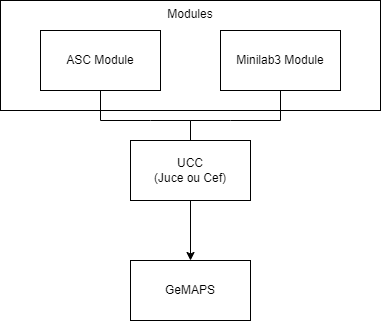
\includegraphics[width=0.5\textwidth]{graphics/gmaps.png}
	\begin{tiny}
	\end{tiny}
	\captionof{figure}{Architecture de l'application GeMAPS}
	\label{fig}
\end{center}

\subsubsection{Environnement technique front-end.}

Pour l'environnement technique front-end, j'ai pu prototyper dès le début du stage l'utilisation de différents frameworks Web dans l'application GeMAPS : React, Angular, et Vue.  

Pour développer les prototypes de l'Arturia Software Center et du Midi Control Center, le choix du framework m'a été laissé : je me sentais plus compétant sur Angular TypeScript, car c'était ce que j'avais utilisé durant le stage précédent. Ceci s'est révélé être une erreur, car cela ne correspondait pas à la stack technologique utilisée au sein de l'entreprise, notamment de l'équipe Web qui travaille avec Vue Nuxt. Afin de favoriser la cohérence de l'entreprise, ainsi que pour bénéficier des conseils d'experts dans le framework, il m'a été recommandé de refactoriser les projets en Vue Nuxt. Cette démarche a permis ainsi une meilleur uniformité dans l'entreprise, ainsi qu'une progression plus rapide de mes compétences personnelles. J'ai également adopté les autres charactéristiques d'environnement technique de l'équipe Web, que sont l'utilisation de Tailwind et du PostCSS pour les styles. 

\subsubsection{Environnement pour la gestion de projet}
L'équipe Compagnon utilise Trello pour la gestion de projet. L'équipe s'en sert pour gérer les tickets, distribuer les tâches, visualiser les tâches en attente de chaque projet ainsi que les tâches en cours.

\subsection{Propositions techniques / Implémentations}
\subsubsection{Prototypage d'utilisation de framework Web}
Mes premières tâches à Arturia fûrent de démontrer la possibilité d'utiliser différents frameworks Web dans l'application GeMAPS.
J'ai ainsi pu réaliser, en Vue, React et Angular, la reproduction d'un page de l'Arturia Software Center, ainsi que les afficher dans une page principale basique, permettant de naviguer entre les pages Web distribuées. 

Les résultats de ce prototypage ont révélé que peu de différences importantes étaient observables entre ces différents frameworks une fois l'application Web compilée. Le point de différence majeur fut que l'architecture de fichiers compilés n'est pas la même par défault sur ces différentes technologies, et nécessite donc de lister les fichiers et répertoires à distribuer pour le serveur de fichiers de GeMAPS.

% \begin{figure}%
%     \centering
%     \subfloat[\centering ]{{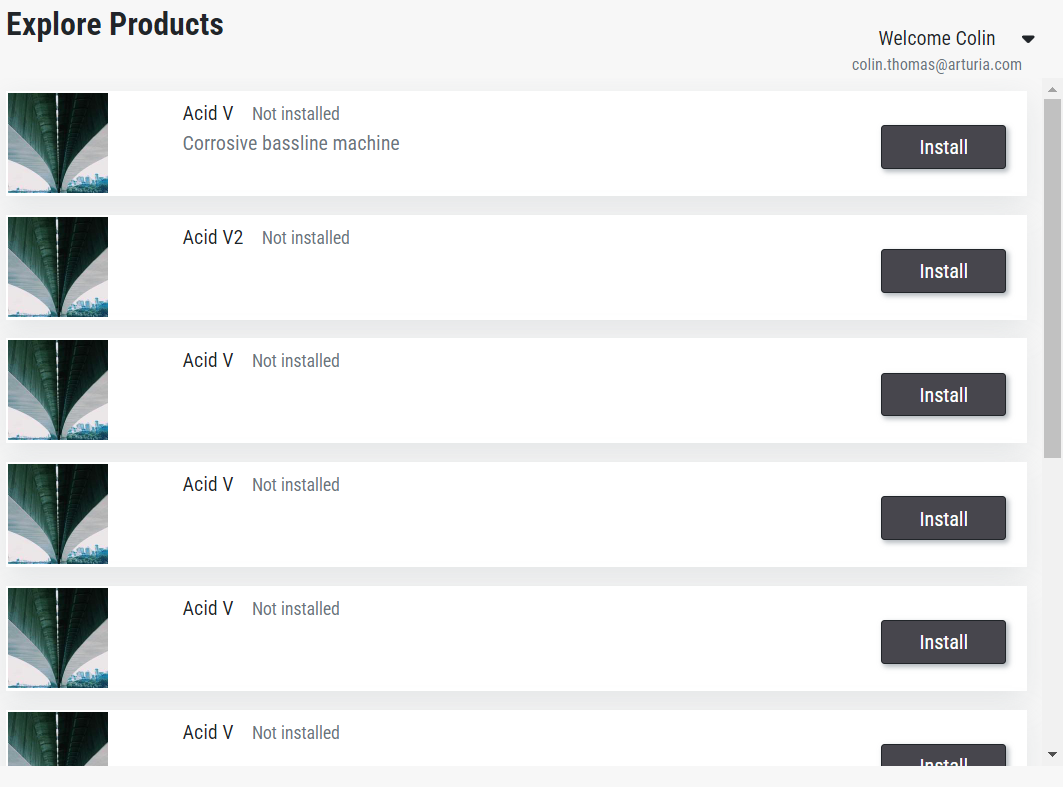
\includegraphics[width=6cm]{graphics/vue_demo.png} }}%
%     \qquad
%     \subfloat[\centering ]{{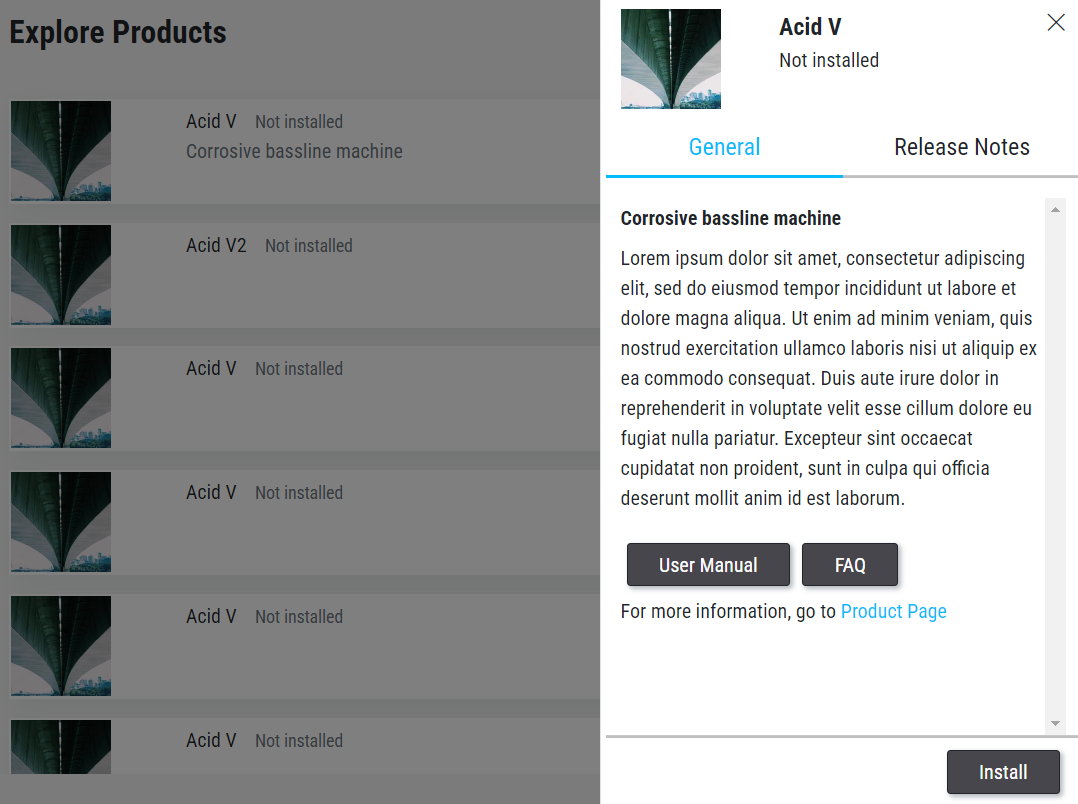
\includegraphics[width=6cm]{graphics/vue_demo2.png} }}%
%     \caption{Page utilisée pour démontrer l'utilisation de différents frameworks dans GeMAPS}%
%     \label{fig:example}%
% \end{figure}
\begin{center}
    \centering
    \begin{minipage}{.5\textwidth}
    \centering
    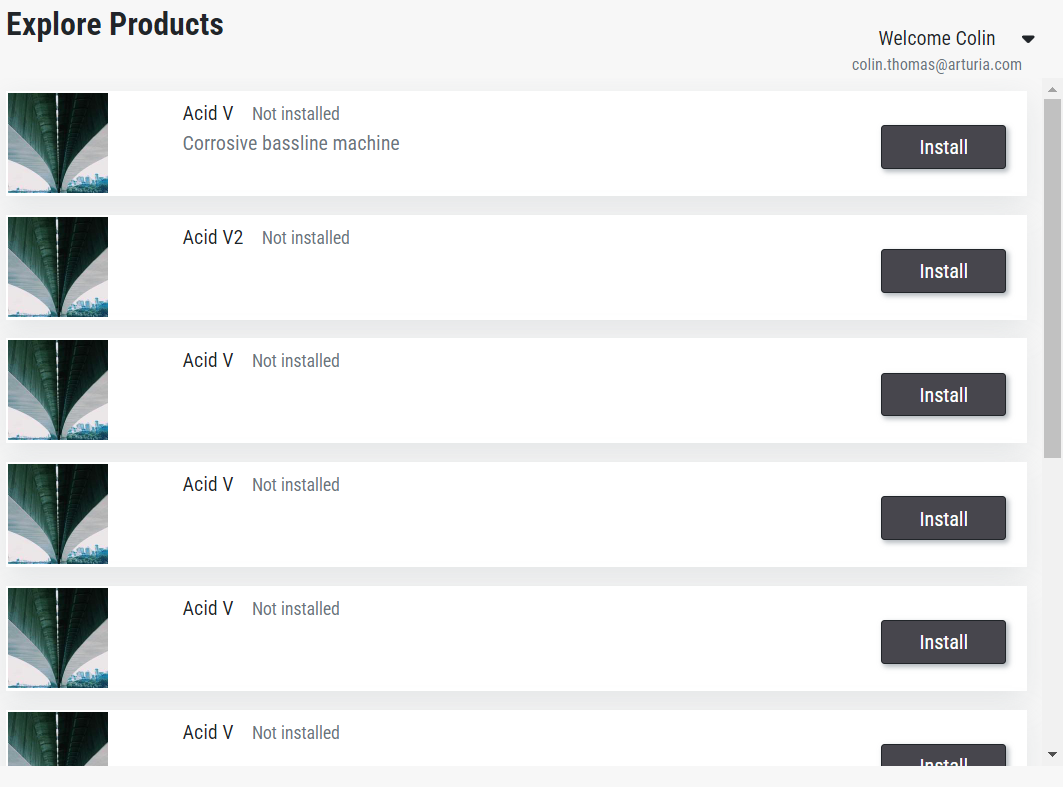
\includegraphics[width=6cm]{graphics/vue_demo.png}
    \label{fig:test1}
    \end{minipage}%
    \begin{minipage}{.5\textwidth}
    \centering
    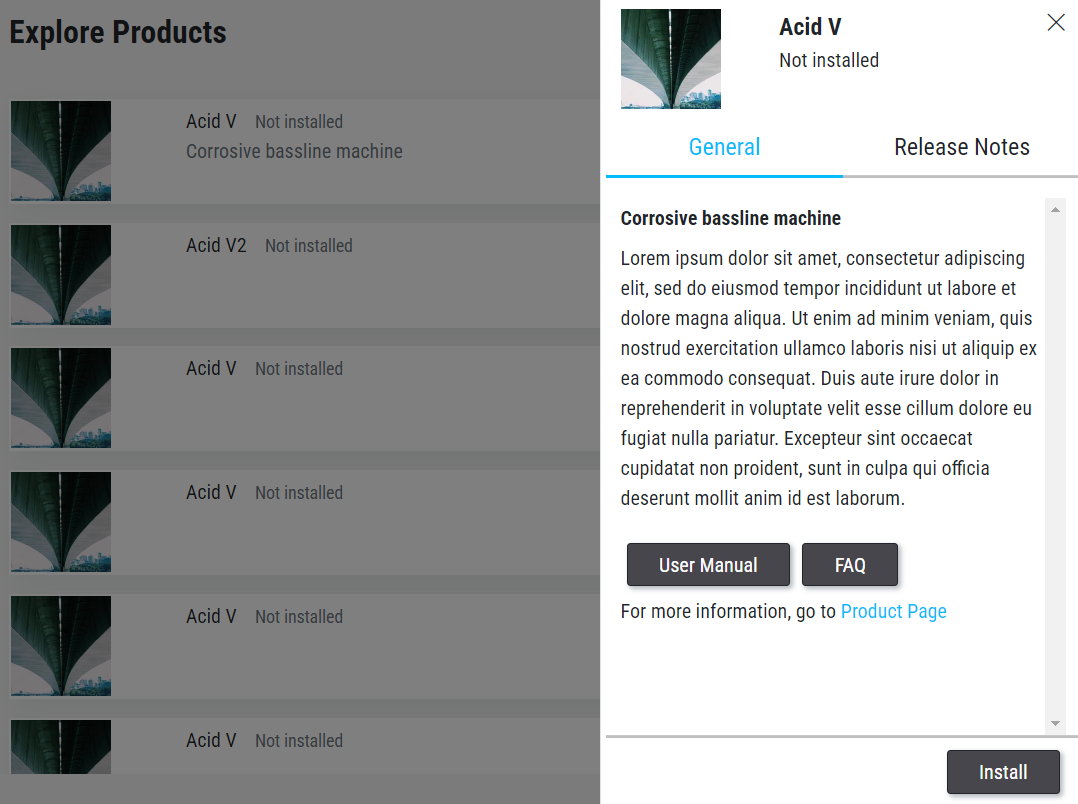
\includegraphics[width=6cm]{graphics/vue_demo2.png}
    \label{fig:test2}
    \end{minipage}
    \captionof{figure}{Page utilisée pour démontrer l'utilisation de différents frameworks dans GeMAPS}%
    \end{center}

Dans le cas d'un serveur Web classique, lorsqu'un navigateur demande une page sans extension, par exemple www.page.com/chemin, le serveur servira automatiquement le fichier www.page.com/chemin/index.html s'il existe. Dans notre cas, nous ne souhaitions pas fonctionner ainsi, car notre serveur sert aussi bien les pages web que les endpoint du back-end, et notre manière pour séparer les endpoint back-end des fichiers web, était l'extension du fichier présente pour ces derniers. 
    
    Cependant, le problème se complexifie dans le cas de Vue Nuxt, car celui-ci utilise une sur-couche de navigation, qui ne reconnait que les chemins sans la partie finale /index.html. Le résultat produit était que le serveur refuse de servir une page si elle ne termine pas par /index.html, mais lorsqu'on le rajoute, Vue Nuxt refuse l'accès.

    La solution de contournement que nous avons choisi, est un middleware intégré au code du front-end : à chaque atterrissage sur une nouvelle page terminant par /index.html, le chemin sera changé en retirant ce suffixe.






\subsubsection{Fonctionnement de la page principale}

L'architecture de la page principale se présente ainsi :

\begin{center}
    \centering
    \centering
    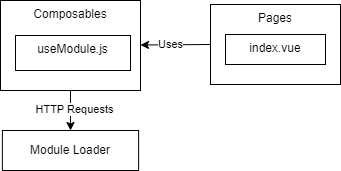
\includegraphics[width=8cm]{graphics/uccnuxt.png}
    \label{fig:test1}
    \captionof{figure}{Architecture de la page principale de GeMAPS (UCC)}%
\end{center}

Ici, le \textit{Module Loader} représente l'élément du back-end de GeMAPS qui met à disposition des endpoints permettant de connaître les modules disponibles.

Au démarrage de l'application, l'application servant de navigateur affiche la page principale du UCC, que l'on va appeler la page Unified Control Center (UCC).

Cette page principale comporte un menu de côté dépliable, qui montre la liste des modules qu'on affiche dans l'application. Chaque module est chargé dans une iframe cachée. En cliquant dessus, on rend visible l'iframe concernée, et on affiche ainsi l'interface sélectionnée.

Ce menu de côté est rempli au démarrage de l'application : la page principale requête le serveur pour déterminer quels sont les end-points où une ou plusieurs interfaces sont disponibles. Ensuite, elle requête le fichier de configuration de ces interfaces Web, et y trouve ses pages à afficher, leurs logos, leurs noms et leurs URLs correspondantes. Enfin, elle affiche une carte dans le menu de côté pour chaque interface, pêrmettant ainsi à l'utilisateur de naviguer facilement entre les modules.



\begin{center}
    \centering
    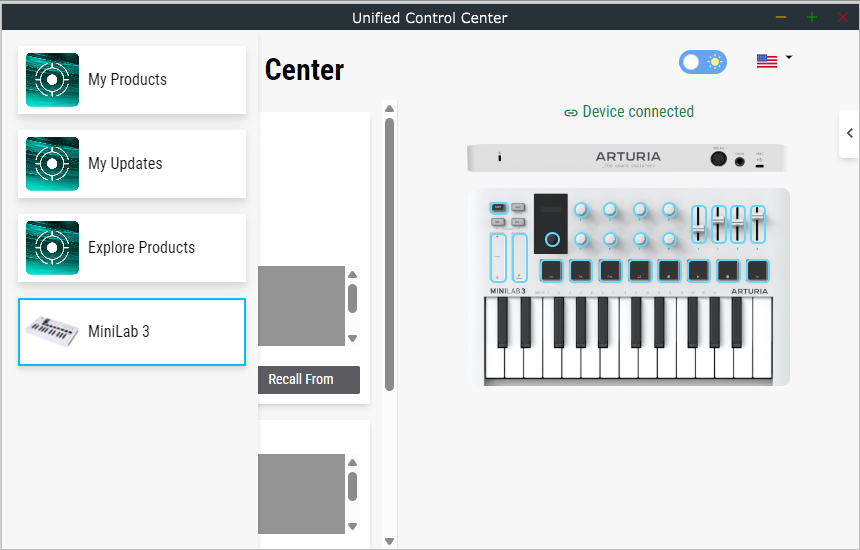
\includegraphics[width=8cm]{graphics/menu_deplie.png}
    \label{fig:test1}
    \captionof{figure}{Unified Control Center avec le menu de côté déplié et le MCC sélectionné}%
    \end{center}

Chaque interface décrite dans le fichier de configuration de chaque module est ainsi ouverte dans une iframe à l'intérieur de la page UCC.

Ouvrir les iframes de chaque module à l'avance et cacher sans fermer les iframes non sélectionnées a été une décision prise dans le but de pouvoir charger les pages au préalable afin d'éviter une attente inutile à l'utilisateur à chaque fois qu'il veut changer de module : par exemple, le Midi Control Center chargera les paramètres du clavier branché, et l'Arturia Software Center synchronisera les licences de l'utilisateur.

\subsubsection{Architecture Web de l'Arturia Software Center}

L'architecture des interfaces Web de l'Arturia Software Center est organisée de la manière suivante : 

\begin{center}
    \centering
    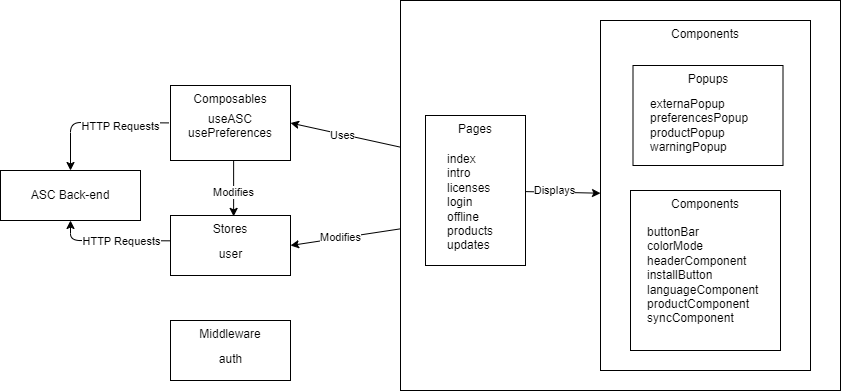
\includegraphics[width=13cm]{graphics/ascnuxt.png}
    \label{fig:test1}
    \captionof{figure}{Architecture de l'interface Web de l'Arturia Software Center}%
\end{center}

Les pages représentent les pages Web que l'on peut visiter : ici, les pages \textit{licenses}, \textit{products} et \textit{updates} sont les onglets affichés par GeMAPS une fois connecté. Les pages \textit{login} et \textit{offline} sont accessibles si l'utilisateur n'est pas connecté, et la page \textit{intro} s'affiche au moment de la première connexion de l'utilisateur, dans le but de lui présenter l'Arturia Software Center.

Les composants sont des éléments affichés par les pages. Parmis les plus importants, le \textit{productComponent} est l'élément de carte contenant les informations réduites des produits lorsque l'on affiche une liste de produits, et la popup \textit{productPopup} est la popup qui affiche les détails d'un produit lorsqu'on le sélectionne.

Les composables sont des éléments de processing, appelables par les pages, les composants, ou d'autres composables. Ici, \textit{useASC} est le composable principal de communication avec le back-end, tandis que le composable \textit{usePreferences} communique avec le back-end à propos des préférences de l'utilisateur.

Le store \textit{user} contient les informations utilisateur, que sont le nom ou l'e-mail utilisateur, mais également la logique de connexion ou déconnexion et la communication avec le back-end que ceci implique.

Enfin, le middleware \textit{auth} sert de composant logiciel intermédiaire entre le navigateur et la page Web. Il redirige automatiquement tout utilisateur non connecté vers la page de connection.



\subsubsection{Fonctionnalités clés de l'Arturia Software Center}

\paragraph{La connexion utilisateur}: La connexion utilisateur comporte ici plusieurs points de complexité. 

En effet, la connexion de l'Arturia Software Center déjà existant inclut la synchronisation, c'est à dire le moment où le back-end vérifie que toutes les images et descriptions de produits sont prétéléchargées, récupère les dernières versions de logiciels mis à jour, et récupère les licenses actuellement possédées par l'utilisateur. Tout ceci se produit après que l'utilisateur ai entré un identifiant et un mot de passe correct : on affiche alors une page de synchronization pour le faire attendre. S'est alors posée pour nous la question de l'implémentation dans une architecture où l'on a séparé le back-end et le front-end : comment prévenir le front-end que la synchronization s'est terminée ? Nous avons opté pour l'utilisation de Server-Sent Events (SSE). Ainsi, lorsque l'utilisateur se connecte, sa requête ne reçoit pas de réponse avant la fin de la synchronisation. En revanche, l'avancement de la synchronisation est partagée entre le back-end et le front-end par SSE (\textit{Server-Sent Events}) envoyés par le back-end, prévenant soit du début, soit de la réussite, soit de l'échec de la synchronisation.
\begin{center}
    \centering
    \begin{minipage}{.5\textwidth}
    \centering
    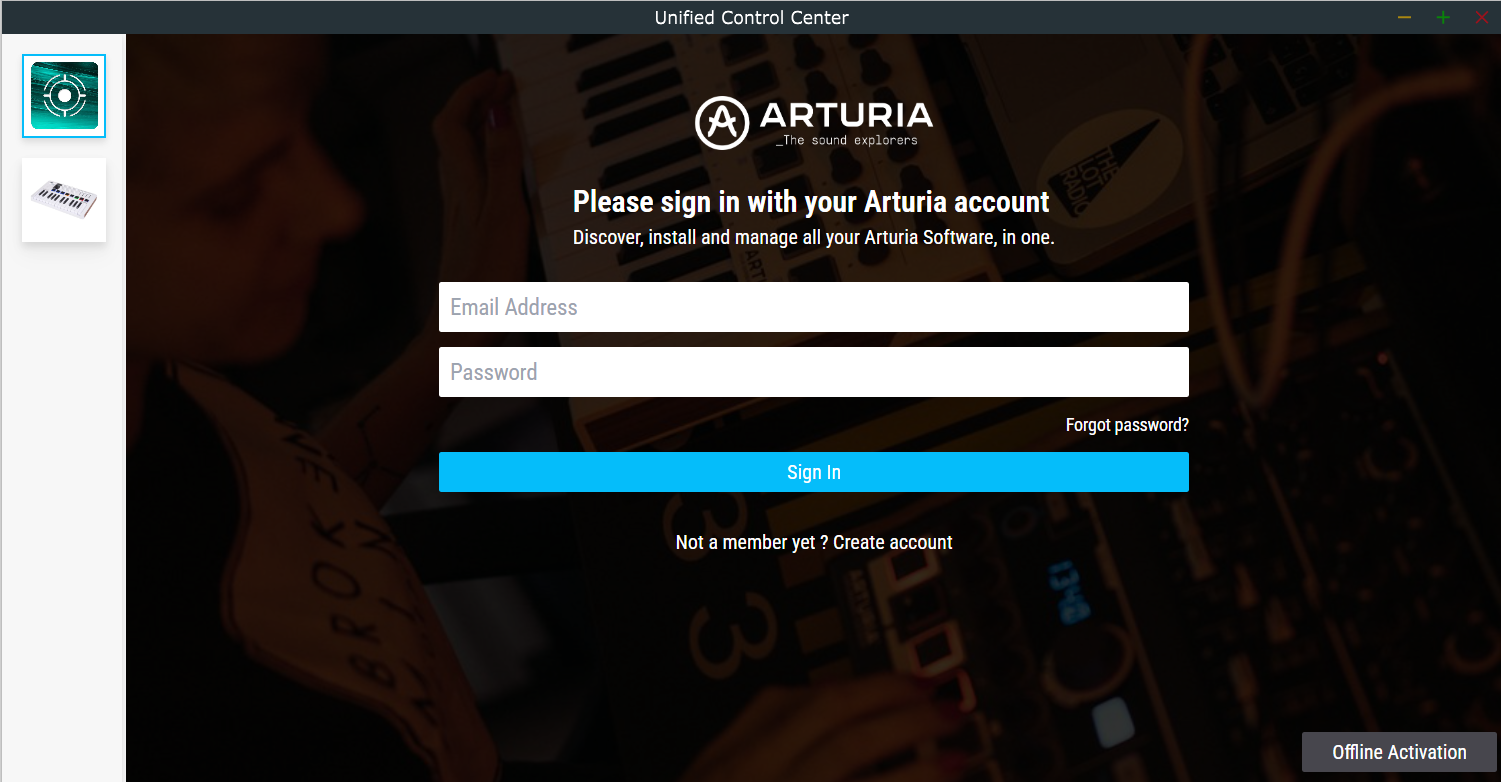
\includegraphics[width=7cm]{graphics/disconnected.png}
    \captionof{figure}{Page de connexion de l'ASC}%
    \label{fig:test1}
    \end{minipage}%
    \begin{minipage}{.5\textwidth}
    \centering
    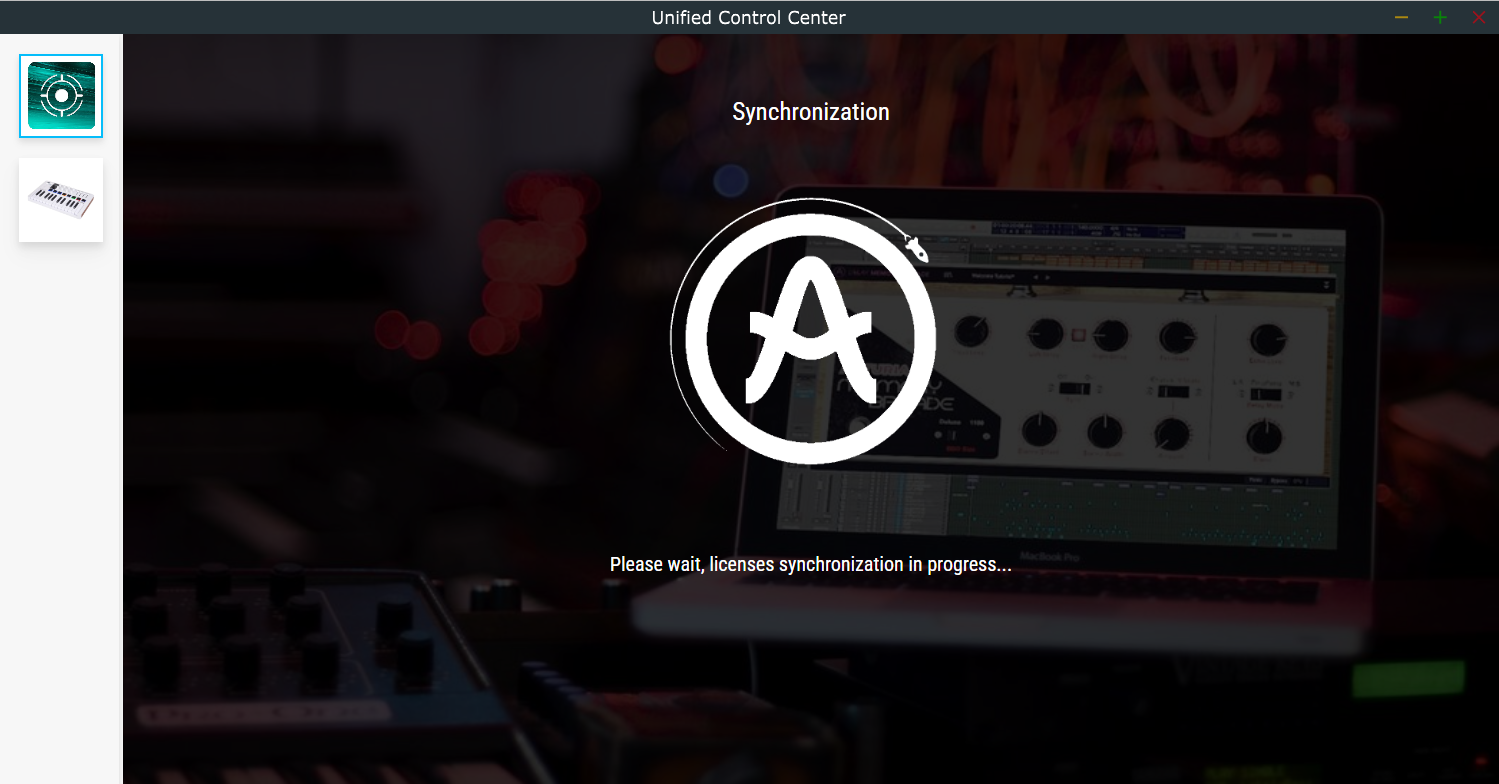
\includegraphics[width=7cm]{graphics/sync.png}
    \captionof{figure}{Page de synchronisation de l'ASC}%
    \label{fig:test2}
    \end{minipage}
    \begin{minipage}{.5\textwidth}
    \centering
    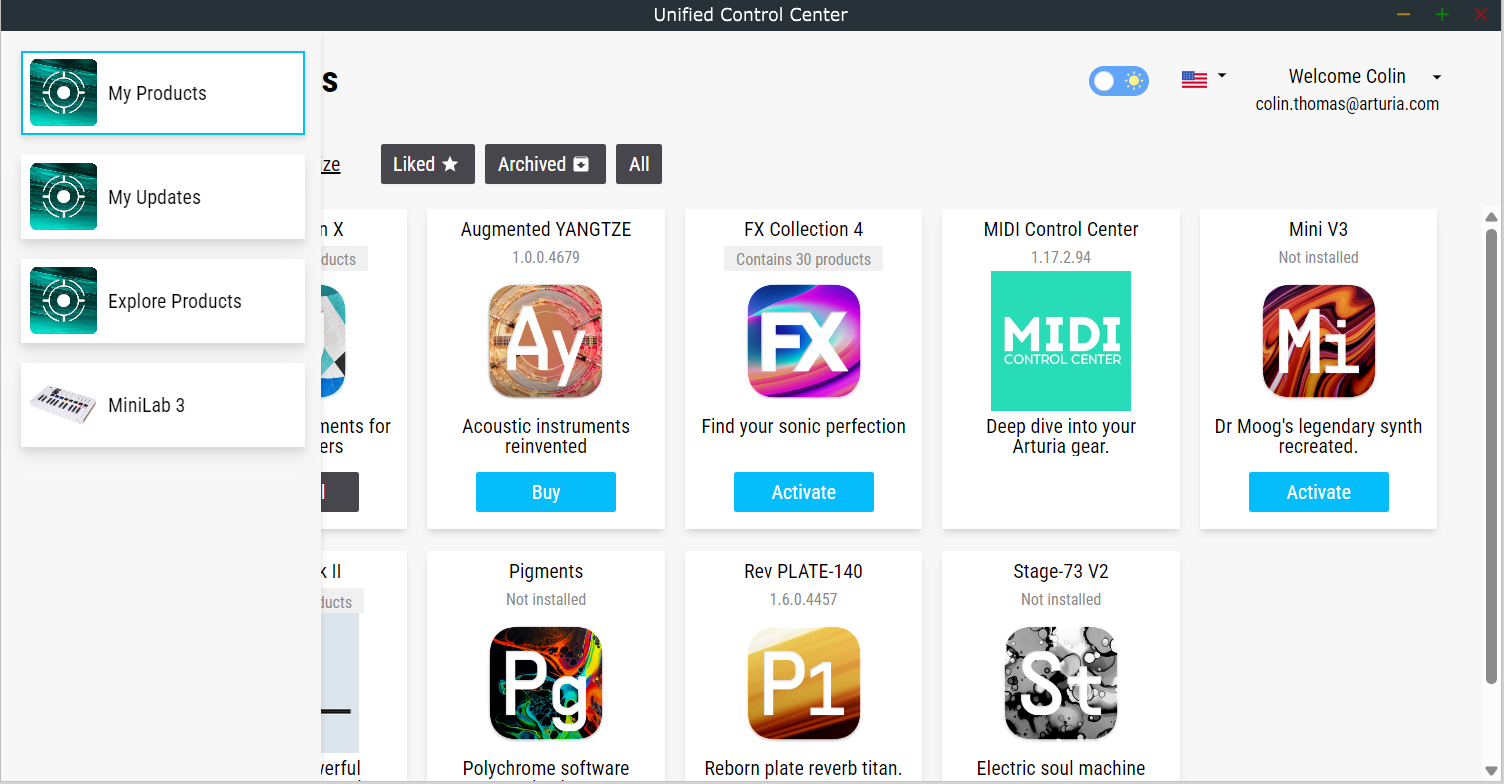
\includegraphics[width=7cm]{graphics/connected.png}
    \label{fig:test2}
    \end{minipage}
    \captionof{figure}{Effet du statut de connexion sur la page principale de GeMAPS}%
\end{center}

Nous avons rencontré un autre défi avec la fonctionnalité de l'auto-login, qui est implémentée par l'Arturia Software Center existant, et qui permet à l'utilisateur de n'avoir à se connecter qu'une fois sur sa machine. Dans notre cas, puisque nous démarrons le back-end et le front-end en même temps, il est crucial pour le front-end de savoir à quel étape de la connexion se trouve le back-end pour afficher les pages correspondantes. Pour résoudre ce problème, nous avons décidé d'ajouter un endpoint au back-end, qui permet, en cas d'auto-login, de demander si l'utilisateur est en cours de connexion, de synchronisation, ou si tout est déjà terminé.

Enfin, il était illogique d'un point de vue de l'expérience utilisateur d'avoir 3 pages disponibles pour les 3 onglets de l'Arturia Software Center, même si ceux-ci sont déconnectés. L'utilisateur voyait de cette façon 3 fois la même page de connexion. Pour y remédier, nous avons décidé de ne rendre disponible qu'une page de connexion sur la page principale de GeMAPS, tant que l'utilisateur n'est pas connecté. Ceci nécessite ainsi de partager le statut de connexion entre la page Web principale, et la page Web de l'Arturia Software Center. Pour ce faire, nous avons décidé de passer par le stockage local de navigateur. 


\paragraph{Installation de produits} A COMPLETER
\paragraph{Fonctionnalité multilingue}: Le multilingue est une fonctionnalité essentielle pour Arturia, et est en cours de développement dans plusieurs projets. La facilité de développement multilingue qu'amène la technologie Web est un autre avantage que montre mon prototype.

Pour développer cette fonctionnalité, j'ai utilisé les mêmes technologies que l'équipe Web d'Arturia.En effet, comme mentionné précedemment, l'équipe de développement Web d'Arturia a déjà mis en place un système complexe de traitement des traductions, et travailler de manière uniforme avec eux permettra ainsi de s'intégrer à leur processus de traduction. 

J'utilise ainsi le package @nuxtjs/i18n. En pratique, cela me permet, dans chaque composant ou page Web, de remplacer chaque texte à traduire par un identifiant qui lui est propre. Ensuite, j'écris au format JSON le texte auxquel correspond chaque identifiant, en français et en anglais.

Pour passer d'une langue à l'autre, j'ai créé un composant qui permet de choisir entre les langues disponibles.

\begin{center}
	\centering
	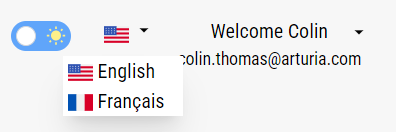
\includegraphics[width=5cm]{graphics/languages.png}
	\begin{tiny}
	\end{tiny}
	\captionof{figure}{Composant de selection de langue}
	\label{fig}
\end{center} 

Une fois le projet compilé pour la production, toutes les pages existent en autant d'exemplaire qu'il y a de langues disponibles : ainsi, par exemple, la page \textit{login/index.html} française est disponible à l'adresse \textit{fr/login/index.html}

\paragraph{Mode sombre}: Pareillement que le multilingue, le Mode sombre est une fonctionnalité commune et très documentée en technologies Web. Pour le développer, j'ai utilisé l'attribut de Tailwind PostCSS pour créer un style sombre pour chaque page et composant Web, et j'ai créé un composant permettant de sélectionner le mode voulu, que j'ai ajouté au header. 

De même que pour la connexion, je partage cet élément par le stockage local du navigateur, afin que toutes les fenêtres de GeMAPS, ainsi que la fenêtre hôte, passent en mode sombre lorsqu'il est déclenché sur un module.

\begin{center}
    \centering
    \begin{minipage}{.5\textwidth}
    \centering
    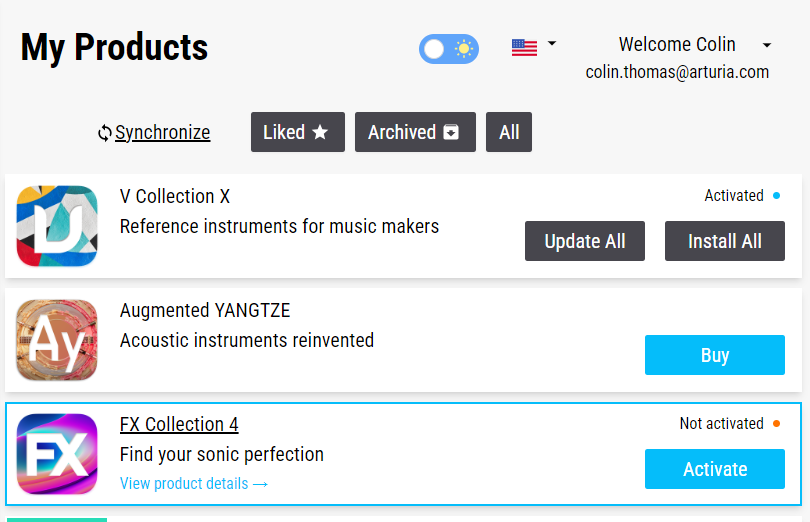
\includegraphics[width=7cm]{graphics/daymode.png}
    \label{fig:test1}
    \end{minipage}%
    \begin{minipage}{.5\textwidth}
    \centering
    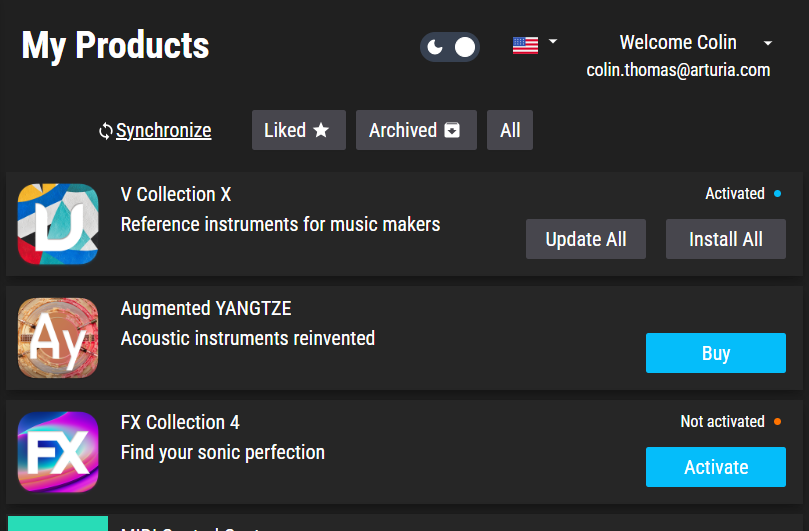
\includegraphics[width=7cm]{graphics/darkmode.png}
    \label{fig:test2}
    \end{minipage}
    \captionof{figure}{Effet du Mode sombre sur l'ASC}%
    \end{center}


\paragraph{Favoris et Archivés}: 
Une des fonctionnalités qui m'ont été demandé pendant mon développement, a été de créer des catégories Favoris et Archivés pour les produits : en effet, en possédant de nombreux produits Arturia, la liste peut être longue, et il peut être fastidieux de naviguer longtemps pour chercher un produit qu'on utilise souvent.

J'ai ainsi ajouté une barre de boutons Favoris, Archivés et Tous sur l'Arturia Software Center, afin de pouvoir sélectionner quels produits afficher.
De même, j'ai ajouté des boutons Favoris et Archivés dans la page détails du produit. 
J'ai choisi de développer cette fonctionnalité de la manière la plus modulaire possible, afin qu'ajouter une catégorie supplémentaire à 'Favoris' ou 'Archivés' puisse être fait facilement. //TODO : développer

% \begin{center}
%     \centering
%     \begin{minipage}{.5\textwidth}
%     \centering
%     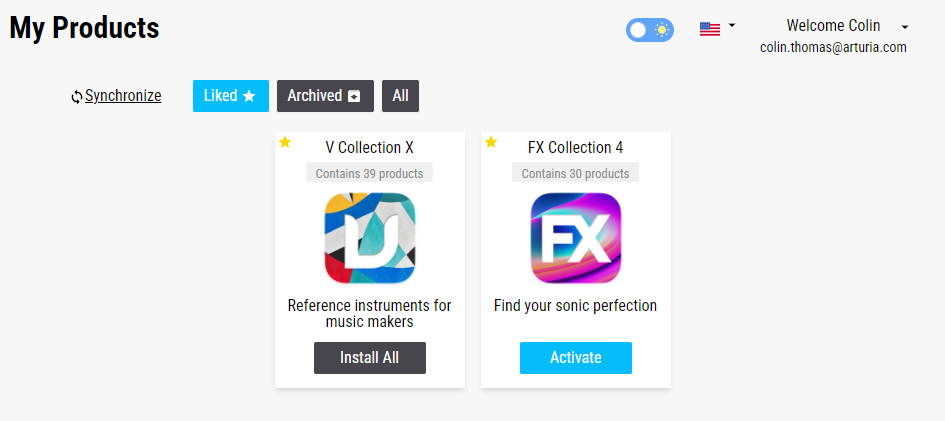
\includegraphics[height=4cm]{graphics/favorite.png}
%     \label{fig:test1}
%     \end{minipage}%
%     \begin{minipage}{.5\textwidth}
%     \centering
%     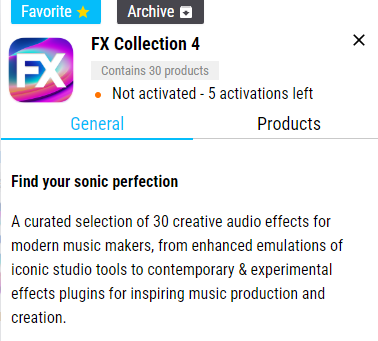
\includegraphics[height=5cm]{graphics/favorite_details.png}
%     \label{fig:test2}
%     \end{minipage}
%     \captionof{figure}{Fonctionnalité Favoris et Archivés}%
%     \end{center}
% Image

\paragraph{Réactivité}: Une autre fonctionnalité très demandée, et facilitée par le Web, a été de faire un affichage dynamique, qui réagit au changement de taille de la fenêtre. En effet, l'Arturia Software Center déjà existant bloque sa taille, et ne peut pas être mis en plein écran.

Pour cette tâche, j'ai mis en place un affichage basé sur des cartes. Ainsi, lorsque la fenêtre est agrandie en largeur, les produits qui dépassent une certaine largeur sont présentés sous forme de grille de cartes.

\begin{center}
    \centering
    \begin{minipage}{.5\textwidth}
    \centering
    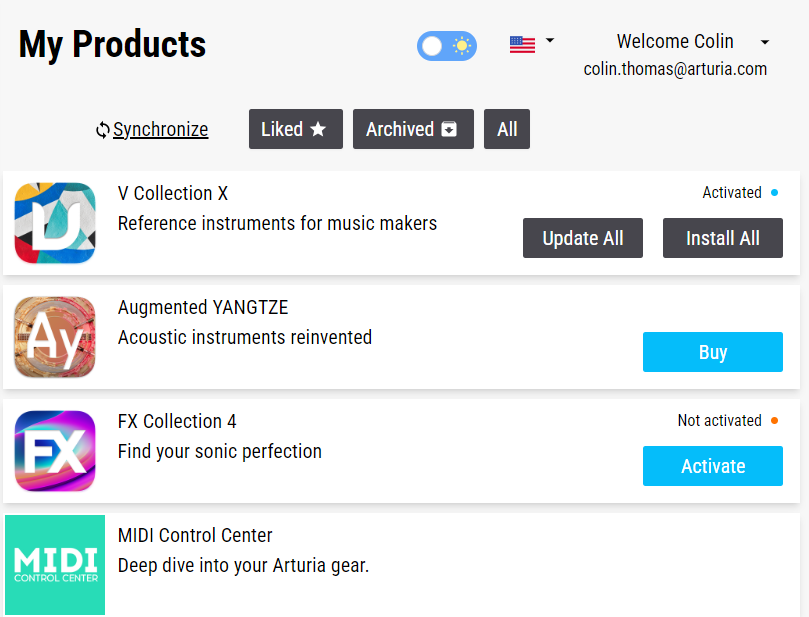
\includegraphics[height=5cm]{graphics/small.png}
    \label{fig:test1}
    \end{minipage}%
    \begin{minipage}{.5\textwidth}
    \centering
    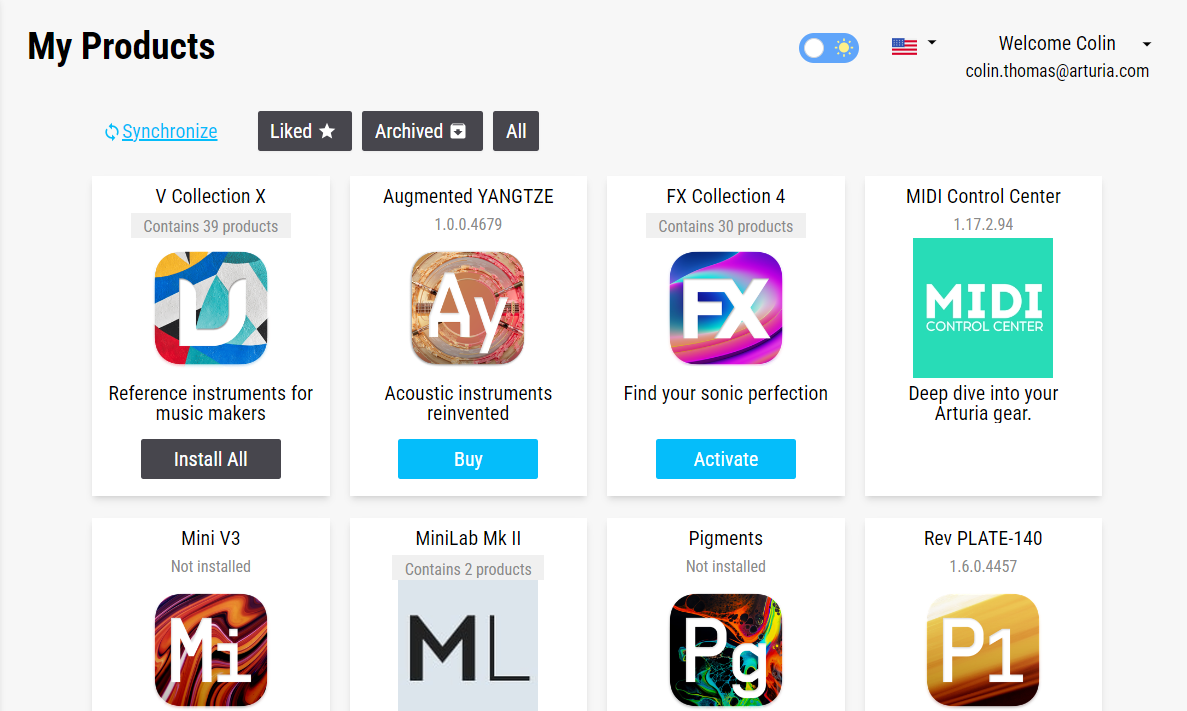
\includegraphics[height=5cm]{graphics/big.png}
    \label{fig:test2}
    \end{minipage}
    \captionof{figure}{Affichage des produits réagissant à la taille de la fenêtre.}%
\end{center}


\subsubsection{Architecture Web du Midi Control Center}

L'architecture des interfaces Web du Midi Control Center est organisée de la manière suivante : 

\begin{center}
    \centering
    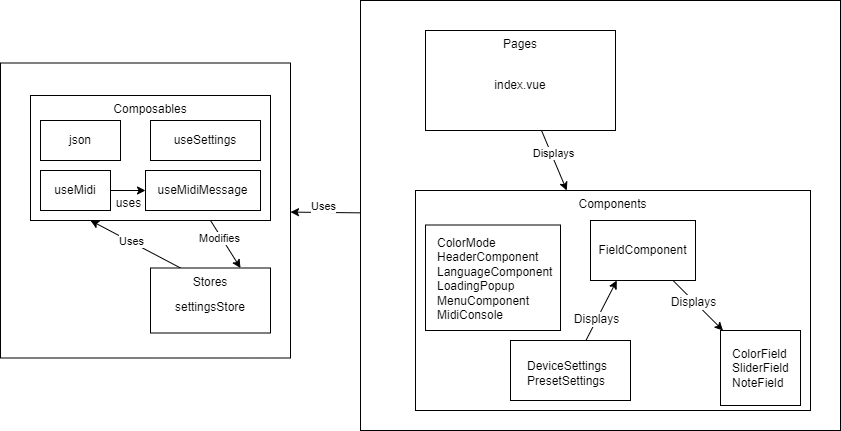
\includegraphics[width=15cm]{graphics/minilab3nuxt.png}
    \label{fig:test1}
    \captionof{figure}{Architecture de l'interface Web du Midi Control Center}%
\end{center}

Cette application Web n'a qu'une seule page.

Les composants \textit{ColorField}, \textit{SliderField} et \textit{NoteField} sont des composants affichant respectivement des champs de sélection de couleur, de valeur sur slider et de note de musique. Il sont utilisés par le plus large \textit{FieldComponent}, lui même affiché dans le composant \textit{DeviceSettings}, affichant les paramètres d'appareil, et \textit{PresetSettings}, affichant les paramètres de préréglage.

Les composables sont utilisés par la page, les composants, les autres composables, et le store. Nous pouvons y retrouver \textit{useJSON}, qui contient des outils de gestion des fichiers de paramètres JSON, comme par exemple la création et le téléchargement d'un objet au format JSON. \textit{useSettings} contient la logique de gestion des settings et de leur envoi et réception au controleur MIDI. \textit{useMidi} contient une logique plus basse, servant de sur-couche à l'API Web MIDI, et \textit{useMidiMessage} contient la logique de traitement et de traduction des messages MIDI, pour déterminer par exemple si c'est un SysEx, quel controle il concerne, ou quel valeur il transporte, mais aussi pour créer un message SysEx à envoyer au contrôleur.

Le store \textit{settingsStore} stocke les paramètres d'appareil et les paramètres de préréglage.



\subsubsection{Fonctionnalités clés du Midi Control Center}

Nous nous sommes ici limités au Midi Control Center appliqué au controleur MIDI MiniLab 3 d'Arturia.

\paragraph{L'API Web MIDI}:
J'ai tout d'abord réalisé une preuve de concept de l'utilisation de l'API Web MIDI, où j'ai réussi à récupérer les touches appuyées et les vélocités du MiniLab 3 entièrement en Web. Ensuite, j'ai également exploré l'utilisation des messages SysEx dans cette preuve de concept pour valider leur fonctionnalité en API Web MIDI.
Après avoir validé leur fonctionnement sur le MiniLab 3, je l'ai ensuite implémenté dans un Midi Control Center complet pour le MiniLab 3. 

Lors de mon utilisation de l'API Web MIDI, j'ai privilégié le développement de composables génériques et réutilisables, afin de permettre une réutilisation facile de mes travaux, ainsi qu'une adaptation rapide pour le Midi Control Center d'autres appareils.


\paragraph{L'API Web USB et l'update Firmware}:
J'ai pu prototyper, pendant mon développement du Midi Control Center, une fonctionnalité d'update firmware des appareils Arturia entièrement en Web. Pour faire ceci, j'ai utilisé l'API Web USB
\footnote{\url{https://developer.mozilla.org/en-US/docs/Web/API/USB}} 
, en m'appuyant sur un projet open-source 
\footnote{\url{https://github.com/devanlai/webdfu}}
implémentant une update firmware DFU Web pour les cartes électroniques STM32.
J'ai d'abord commencé par l'expérimenter sur le MiniLab 3, qui fait partie des produits qui n'ont qu'un micro-processeur à mettre à jour, et est donc plus simple, puis ensuite le MiniFreak, qui possède 6 micro-processeurs à mettre à jour les uns après les autres.

Sur Windows, Arturia utilise un pilote USB MIDI propriétaire, qui lui permet notamment de mettre à disposition ses interfaces MIDI à plusieurs clients en même temps. Ce pilote fut le problème majeur rencontré, car il empêche la mise à jour sur Windows en raison de son incompatibilité avec l'API Web USB, conçu pour le pilote générique WinUSB. J'ai pu tout de même réaliser la mise à jour sur Mac ainsi qu'en remplaçant le driver Arturia par WinUSB sur Windows. Ceci pose cependant un frein à la réalisation d'un Midi Control Center entièrement en technologies Web, car nous ne pouvons pas pour l'instant nous passer de ce pilote dans tous les produits Arturia, et que nous pouvons uniquement l'utiliser en C++.

Cependant, ce prototype reste pertinent, car il permet d'imaginer des possibilités futures sur des produits qui auront un pilote différent.
En effet, plusieurs produits Arturia n'utilisent pas le pilote de l'entreprise, qui communique en MIDI, mais plutôt un pilote USB qui possède une description WinUSB. La raison à cela est double : la communication MIDI est lente, et pose donc problème sur des produits avec beaucoup de paramètres comme le PolyBrute, mais surtout, la communication MIDI est ouverte à tous les logiciels. Ceci veut dire qu'un logiciel de Musique Assistée par Ordinateur, comme Ableton, sur lequel on branche un MiniFreak et auxquel on vient ajouter le plug-in MiniFreak V, peut accèder au port MIDI autant que le logiciel MiniFreak V, et donc potentiellement perturber la communication entre le MiniFreak et son plug-in : ce sont des choses qui ont précédemment posé problème sur plusieurs produits qui ont un plug-in associé.
Le resultat de tout ça est que certains produits, comme le MiniFreak ou le récent AstroLab, n'ont pas de pilote MIDI mais plutôt un pilote USB, et peuvent donc être mis à jour en Web USB même sur Windows.



\begin{center}
	\centering
	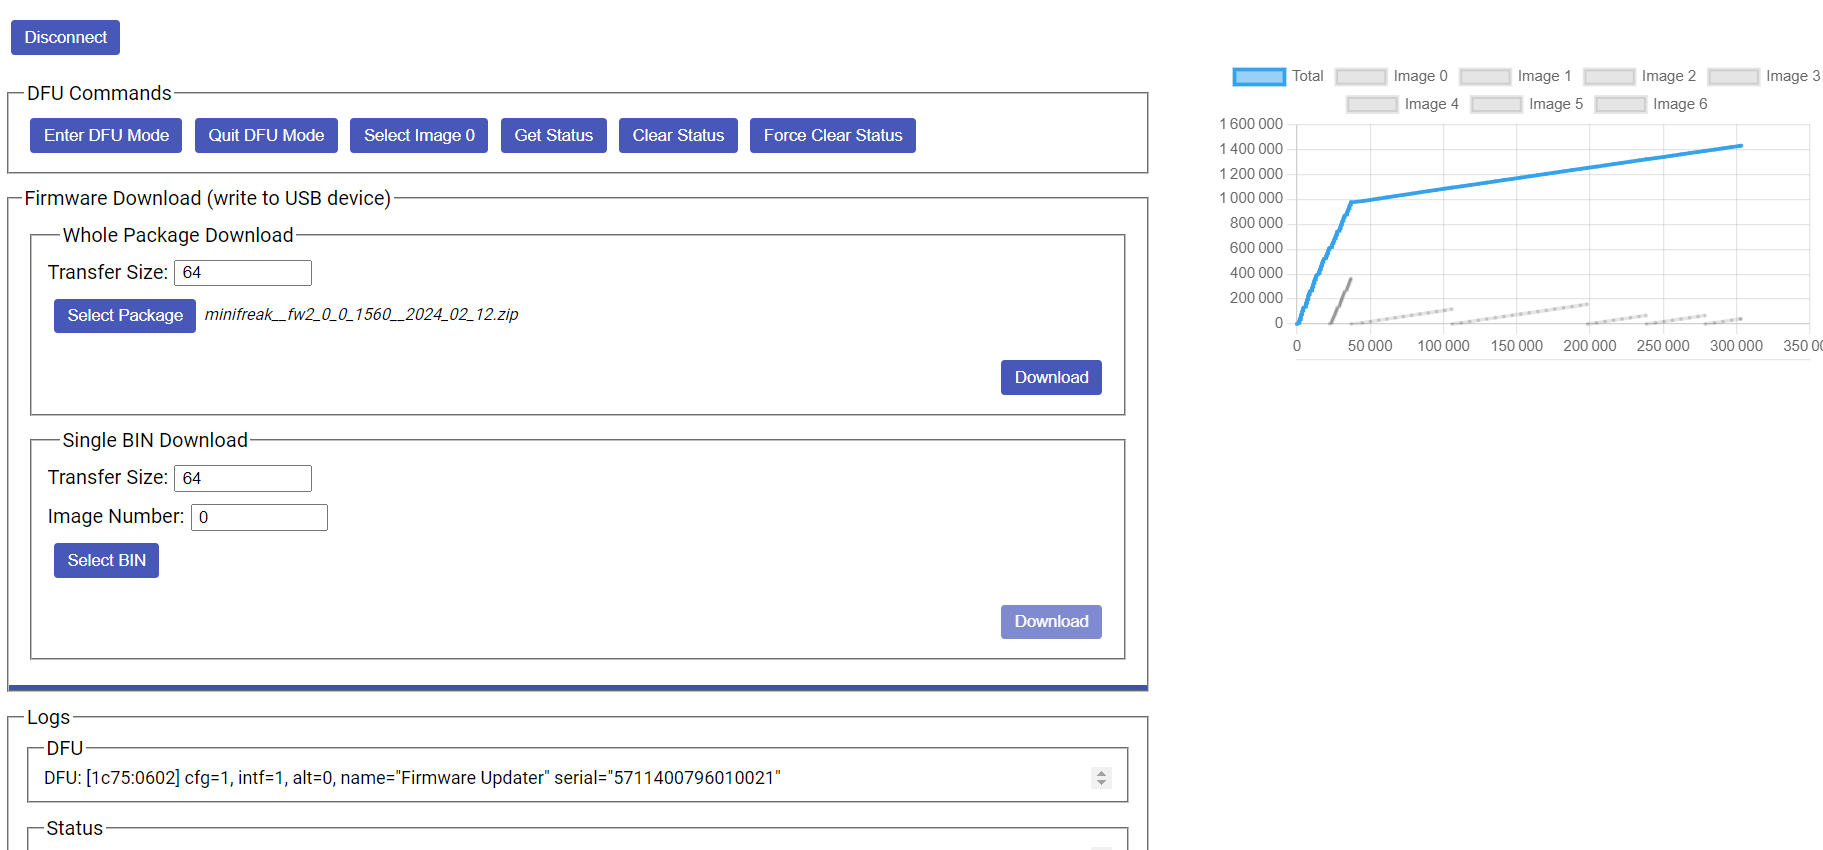
\includegraphics[width=15cm]{graphics/dfu.png}
	\begin{tiny}
	\end{tiny}
	\captionof{figure}{\centering Prototype d'utilisation de l'API Web USB pour l'update firmware DFU}
	\label{fig}
\end{center}


\paragraph{La création d'une nouvelle interface}:
Je me suis ensuite lancé dans la conception d'un Midi Control Center Web appliqué au MiniLab 3.
Le Midi Control Center possède des interfaces graphiques vieillissantes : contrairement à l'Arturia Software Center, que j'ai recopié comme tel, j'ai cherché à retravailler les interfaces du MCC. Puisque les deux logiciels vont se retrouver dans une seule architecture modulaire, j'ai souhaité uniformiser les visuels entre l'Arturia Software Center et le Midi Control Center.

J'en ai donc repris les couleurs et les polices de charactères. Je me suis également inspiré des cartes avec ombres de l'ASC pour les différents menus du Midi Control Center.

\begin{center}
    \centering
    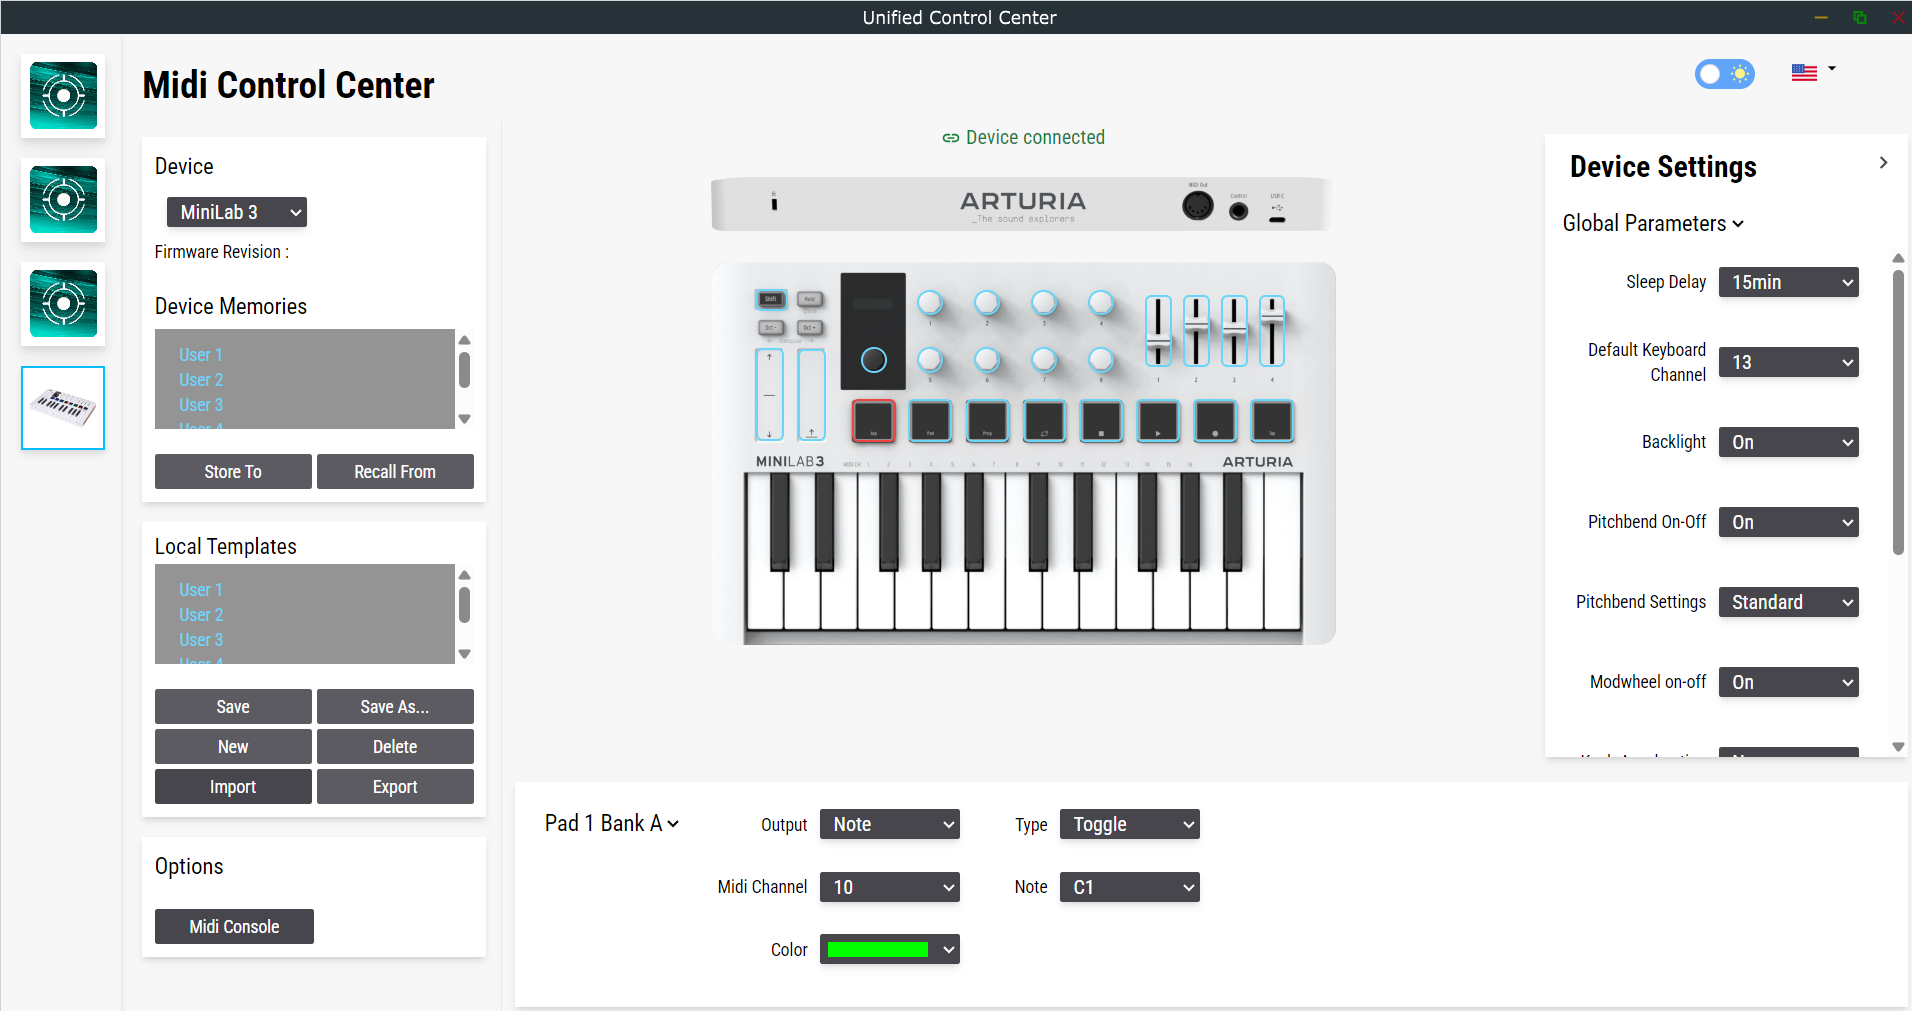
\includegraphics[width=10cm]{graphics/mcc_new.png}
    \captionof{figure}{\centering MCC retravaillé pour être uniforme avec l'ASC.}
    \label{fig:test1}
\end{center}

On peut remarquer ici les boutons bleus alignés sur les controles du MiniLab 3 : ils permettent de sélectionner de quel controle nous souhaitons modifier les paramètres. Dans le Midi Control Center existant, la disposition de ceux-ci se fait sur la base d'un fichier JSON qui précise l'identifiant de chaque controle, son emplacement, sa forme et sa taille. C'est donc sur ce fichier là que je récupère la disposition de tous les contrôles. Cependant, les tailles et emplacements sont renseignés en pixels, ce qui ne convient pas à mon fonctionnement réactif au redimensionnement de la page : je récupère donc la taille en pixels de l'image, et je traduis toutes les tailles et emplacements des contrôles en pourcentages de l'image : de cette manière, l'image du contrôleur et ses contrôles se redimensionnent correctement en fonction de la taille de la fenêtre.



\paragraph{La gestion des paramètres de l'appareil}:

Tous les paramètres du MiniLab3 sont stockés dans le Store de l'application Web.

\begin{itemize}
    \item Paramètres d'appareil :  Tout comme le faisait Midi Control Center déjà existant, les paramètres d'appareil sont chargés au branchement du MiniLab 3. De même, à chaque changement de valeur d'un paramètre d'appareil, un message SysEx est envoyé au MiniLab 3 pour opérer ce changement.
    \item Paramètres de préréglage : Par rapport aux paramètres de préréglage, nous opérons également en suivant la méthode du Midi Control Center actuel : nous pouvons ainsi importer et exporter tout les paramètres de préréglage de chaque profil sur le controleur. 
    
    Cependant, la sauvegarde des paramètres sur l'ordinateur pose problème : elle est impossible en Web car cela poserait des problèmes de sécurité. Ainsi, nous avons conceptualisé, avec l'équipe Compagnon, un module sans interface Web, qui servirait de système de fichiers. Il aurait un end-point pour importer un fichier, et un autre pour exporter. Créer ce module sans interface plutôt qu'intégrer cette fonctionnalité au back-end du MCC MiniLab 3 permettrait de créer un module générique utilisable par tout autre module Web ayant besoin du système de fichiers. En attendant le développement d'un tel service, j'ai réalisé une importation par sélection de fichier, et une exportation en téléchargement dans le dossier par défaut de téléchargement du navigateur.
\end{itemize}

Lors de l'importation de paramètres, nous envoyons le SysEx demandant ce paramètre en particulier, puis nous attendons la réponse de l'appareil. En cas de non réponse, nous renvoyons le SysEx 2 fois de plus avant de déclarer une erreur.

Cette méthode d'envoi séquentiel de SysEx, en attente de réponses avant d'envoyer les suivants, convient au MiniLab 3 en raison de son nombre limité de paramètres. Pour un appareil avec plus de paramètres, nous pouvons également envisager d'envoyer tous les SysEx à la suite sans attendre les réponses, et de traiter les réponses à leur réception.

\paragraph{Fonctionnalités supplémentaires}:
J'ai implémenté dans ce Midi Control Center la fonctionnalité multilingue ainsi que le mode sombre, de la même manière et avec les mêmes technologies et composants que pour l'Arturia Software Center.

\subsection{Expérimentations et validations}

Les expérimentations et validations ont été une partie importante de mon projet de fin d'études.

Comme mentionné précédemment, j'ai réalisé plusieurs preuves de concept préalables au développement des prototypes d'Arturia Software Center et de Midi Control Center.

Parmi elles, j'ai pu expérimenter l'utilisation de GeMAPS pour distribuer différents frameworks (Vue, React et Angular), et vérifier leur bon fonctionnement. J'ai choisi volontairement, pour réaliser cette expérimentation, une page Web comportant plusieurs éléments clés, comme une pop-up provenants de packages extérieurs, des images ou des éléments scrollables.

J'ai pu également expérimenter l'utilisation des API de Web MIDI et de Web USB.
Pour le Web MIDI, j'ai réalisé une page Web capable d'afficher les contrôles saisis sur le contrôleur midi, et capable d'envoyer des informations SysEx et de réclamer des valeurs SysEx. J'ai pu ainsi rapidement réaliser qu'aucun obstacle ne se posait à l'utilisation du Web USB dans un Midi Control Center en technologies Web.
Pour le Web USB, j'ai développé une page capable de mettre à jour les appareils Arturia en DFU. J'ai pu remarquer et comprendre les obstacles à l'utilisation de cette technologie dans le cadre du fonctionnement actuel de la communication USB à Arturia, et ai pu comprendre ses enjeux pour les appareils futur.

Certains outils m'ont été utiles pour la validation du bon fonctionnement de ce que je produisais. Un outil qui m'a souvent permis de valider ce que me renvoyait le back-end, pour vérifier que j'affichais réellement ce qui correspondait, est Postman. J'ai réalisé une collection de requêtes correspondant à toutes les requêtes possibles à faire au back-end, et cela m'a permis souvent de comprendre d'où venait ce qui me posait problème : en remontant à la source de la requête, j'ai pu séparer les instants où mes interfaces Web ne répondaient pas de la bonne façon, des instants où le back-end n'avait pas une réponse correspondant aux besoins du front-end. De plus, Postman m'a permis de tester plus en profondeur le système de connexion et déconnexion : en étant capable d'envoyer un signal de déconnexion à tout moment au back-end, on est ainsi capable de tester plus de cas possibles d'états de connexion.

Par ailleurs, le navigateur intégré du framework C++ JUCE, que nous utilisons pour afficher l'Unified Control Center, est capable d'afficher une console, ainsi que de laisser accès à son stockage local. Ceci m'a permis de modifier le stockage local en cours de fonctionnement de l'application, ainsi que de vérifier certaines valeurs par la console, ce qui a grandement aidé à la robustesse des projets sur lesquels j'ai travaillé.

Enfin, j'ai pu tester et valider de nombreux cas de renvois d'erreurs ou de renvois non conformes d'informations par le back-end, en le simulant à l'aide du répertoire \textit{server} de mes projets Vue Nuxt, qui permet de produire des maquettes d'endpoints qui sont automatiquement mis à disposition lorsque le projet est lancé en mode développement.

\section{Bilan personnel}
\subsection{Acquis}
\subsubsection{Acquis techniques}

Mon projet de fin d'études à Arturia n'est pas terminé, mais est déjà une expérience formatrice et qui m'a permis de beaucoup monter en compétences. 

J'ai non seulement eu l'occasion d'approfondir mes compétences de développement Web acquises lors de mon stage précédent, en découvrant Vue Nuxt, ainsi qu'en profitant des revues de code que j'ai pu faire avec l'équipe Web d'Arturia pour adopter de bonnes pratiques de développement, mais j'ai pu également monter en compétence sur d'autres domaines très variés. 

Notamment, en assistant et en participant aux réunions d'architecture, j'ai pu réfléchir avec l'équipe Compagnon au fonctionnement d'une architecture novatrice et originale d'application modulaire. J'ai pu également monter en compétences sur la communication MIDI et USB, lors du développement des preuves de concept d'utilisation des API Web MIDI et Web USB, ainsi que plus généralement pendant le développement du Midi Control Center. De plus, l'étude de ces API Web qui sont encore en développement, ainsi que les essais que j'ai pu faire dans le cadre des interfaces Web de GeMAPS, m'ont permis d'approfondir des compétences de créativité et de recherche : contrairement à mes stages antérieurs qui étaient axés principalement sur la production, cette expérience m'a permis de me plonger davantage dans le domaine de la recherche et développement.

J'ai de plus eu l'occasion d'appliquer quelques modifications mineures au projet GeMAPS et au back-end de l'Arturia Software Center. En effet, le membre de l'équipe qui développe ceux-ci travaille sur Mac, et j'ai eu donc quelques modifications à faire pour pouvoir lancer les projets sur Windows.




\subsubsection{Soft skills}
% Parler du statut de mon projet
% Besoin de présenter
% Besoin de contacter pour les reviews
% Travailler en équipe avec jy
% Statut de recherche de ce qu'on peut faire fait que besoin de communication
\subsection{Difficultés rencontrées}
Je n'ai à aucun moment été bloqué longtemps par un problème durant ce projet de fin d'études, mais j'ai cependant rencontré quelques difficultés : 
\begin{itemize}
    \item L'erreur principale que j'ai commise durant ce stage a été de débuter mon projet avec un langage que personne ne maîtrisait ni n'utilisait au sein de l'entreprise.
\end{itemize}
% API Web USB
% Installation et Windows et tout
% Refacto nuxt
% Demande d'aide pour le web
% Communication entre les fenetres ????
% La connexion ASC ??
% Globalement travailler sur quelque chose de nouveau et pas documenté
% En gros pas trop trop de difficultés quoi
% 

\subsection{Retour sur mes attentes}
% surpris sur la pluralité de sujets, de themes et de compétences de mon stage
% surpris de la liberté qu'on me donne
% bonne ambiance
% milieu musical que je cherchais
% tuteur et équipe qui tue
% travailler sur des produits qu'on aime ca tue
% peur de s'enfermer dans le web => pas enfermé oyeah



\section{Conclusion et perspectives}
\subsection{Conclusion}
% Résumé des compétences et de ce que j'ai fait
% Résumé de mon équipe
% J'ai pu bien évaluer
    % Web MIDI et Web USB
    % Tout est faisable
    % On a une idée beaucoup plus claire de comment faire pour la suite


\subsection{Perspectives}
% Je souhaite rester oui
% En faisant plus de trucs
% occasion de beaucoup apprendre, boite de bonne taille pour ca
% occasion d'apprendre plein de trucs parce que equipe compagnon = plateforme centrale de plein de trucs

% Image 

% Bibliographie
% Annexes éventuelles (en plus des 30 pages demandées)
\bibliographystyle{unsrt}


\begin{thebibliography}{9}

    \bibitem{midi}
      H. M. de Oliveira \& R. C. de Oliveira,
      \textit{Understanding MIDI},
      In: 2017,
      URL: \url{https://arxiv.org/pdf/1705.05322},
      (visited on 10/05/2024)

    \bibitem{sysex}
        Cubase,
        \textit{SysEx Messages},
        In: (),
        URL: \url{https://steinberg.help/cubase_artist/v10.5/fr/cubase_nuendo/topics/midi_editors/midi_editors_sysex_messages_c.html},
        (visited on 11/05/2024)
    
    \bibitem{controller}
        Wikipedia,
        \textit{Audio Control Surface},
        In: (2018),
        URL: \url{https://en.wikipedia.org/wiki/Audio_control_surface},
        (visited on 10/05/2024)

    \bibitem{asc}
        Arturia,
        \textit{Arturia Software Center},
        In: (),
        URL: \url{https://www.arturia.com/support/asc-arturiasoftwarecenter},
        (visited on 10/05/2024)

    \bibitem{mcc}
        Arturia,
        \textit{Midi Control Center},
        In: (),
        URL: \url{https://support.arturia.com/hc/fr-fr/sections/4405740766098-MIDI-Control-Center},
        (visited on 10/05/2024)

    \bibitem{webmidi1}
        Mozilla Developper Web Docs,
        \textit{Web MIDI API},
        In: (2023),
        URL: \url{https://developer.mozilla.org/en-US/docs/Web/API/Web_MIDI_API},
        (visited on 10/05/2024)

    \bibitem{webmidi2}
    Adriano Baratè AND Luca A. Ludovico,
        \textit{Web MIDI API: State of the Art and Future
        Perspectives},
        In: (2022),
        URL: \url{https://air.unimi.it/retrieve/60655569-9189-4ff0-9fa0-5614e342af53/JAES2022.pdf}

    

    \bibitem{webusb1}
        Mozilla Developper Web Docs,
        \textit{Web USB API},
        In: (2023),
        URL: \url{https://developer.mozilla.org/en-US/docs/Web/API/WebUSB_API},
        (visited on 10/05/2024)
    
    
    \bibitem{webusb2}
        Web Plaform Incubarot Community Group,
        \textit{Web USB API specification},
        In: (2023),
        URL: \url{https://wicg.github.io/webusb},
        (visited on 10/05/2024)

    
    
    
    \bibitem{webdfu}
        Devanlai (2020) WebDFU [Source code]. \url{https://github.com/devanlai/webdfu}.


    
\end{thebibliography}

\appendix
\section{.}

\end{document}
